\documentclass[a4paper]{article}

\usepackage[margin=1in]{geometry} % full-width
\usepackage{graphicx}
\usepackage[table]{xcolor}
\usepackage{longtable,array}
\usepackage{float}
\usepackage{amsmath}


\graphicspath{{figs/}}

\title{Crucible: An Adversarial, Semi-Cooperative, Dynamic, Scalable, Multi-Paradigm Function Generator for Testing Meta and Hyper Heuristic Optimization Algorithms }

\author{Daniel M. Kennedy$^1$}

\date{
	$^1$University of Central Florida, Orlando, Florida, USA\\ \texttt{da711491@ucf.edu}\\
	\today
}

\begin{document}
	\maketitle


	\begin{abstract}

Standard test cases are useful for experimentation and development of algorithms for finding optimal solutions to wide ranging problems and understanding potential futures. This paper reviews the intersection between optimization, simulation, engineering design optimization, decision analysis, and robust decision making through a lens of optimization under uncertainty and relationships to meta and hyper-heuristic optimization algorithms. A historical review is provided on key features of optimization algorithm benchmarking with a large section devoted to exploring the Congress of Evolutionary Computing (CEC) and Genetic and Evolutionary Computation Conference (GECCO) challenge problems that are frequently used for testing meta-heuristic algorithms. Limitations are identified and used to justify the development of the Crucible Simulation, a scalable, black box, highly configurable, mixed-integer problem requiring pathfinding and single target optimization. Requirements for simulation features are derived and traced to literature references with simulation architecture and features described in detail and traced to requirements. An important contribution of this work is the inclusion of semi-cooperative effects and adversarial, unexpected consequences to optimizer decision making. Three experiments are defined and used to compare performance between the Evolutionary Centers Algorithm (ECA), Particle Swarm Optimization (PSO), Simulated Annealing (SA), and Random Search (RND) algorithms. With all extra simulation features off, SA dominated RND, ECA, and PSO with one network node and many dimensions. However, when all features were on, RND and ECA outperformed SA and PSO. Moreover, in the challenging full featured, four node, four dimension scenarios the high performance of ECA was eroded such that ECA and RND performed equivalently. These results motivate exploring more advanced meta and hyper-heuristic strategies with the Crucible simulation.
		
		\noindent\textbf{Keywords:} Hyper-Heuristics, Meta-Heuristics, Benchmarking, Decision Making, Simulation
	\end{abstract}

%%

\section{Introduction}

%\\- optimization is important in modern complex systems
Simulation and optimization have evolved a synergistic relationship, frequently combined to leverage their strengths to support decision making \cite{fu_handbook_2015}. Optimization is a goal oriented search containing four primary components: input or decision variables, a set of all possible input values, an objective functions with a response, and a stopping criteria to stop the search. The goal of this search is to find the inputs that minimize or maximize the objective function responses, subject to the input constraints \cite{floudas_encyclopedia_2009}. Some examples of quantities and qualities that one might optimize would be the minimization of cost, wait times, or risk, as well as the maximization of profit, efficiency, or throughput.

%\\ starting with opt in general
Early work in optimization includes Fermat's strategy for finding a local minima/maxima of a differentiable function by solving for where the differential is equal to zero, published in 1646. This strategy was generalized to finding the shortest distance to N points by Tedenat and L'Huiller in 1810. Later important breakthroughs were the development of strategies to solve combinatorial optimizations such as Steiner tree problems for finding the shortest path in networks, the simplex algorithm for solving linear programs, as well as advancements in non-linear, integer, stochastic, and dynamic programming \cite{floudas_encyclopedia_2009}.

%\\- what are meta heuristics
Heuristic optimization strategies attempt to find practical solutions over guaranteed globally optimal ones to particular problems. A couple examples of heuristics are greedy and nearest neighbor selection. Meta-heuristic strategies are higher level, problem-independent optimization strategies that are typically constructive, local search, and / or population-based \cite{marti_fifty_2025}. % source: page 1 and 2
Over the last few decades a considerable number of meta-heuristic optimization algorithms have been created and described in literature for tackling especially challenging optimization problems \cite{ma_performance_2023}.
%\\- no free lunch
According to the No Free Lunch theorems \cite{wolpert_no_1997}, optimization algorithms have varying degrees of alignment to different problem classes. If an optimization algorithm outperforms another on average for a class of problems, then it must perform worse on average for the remaining classes of problems.

%\\-- generalization of optimization algorithms
Hyper-heuristic algorithms attempt to address this constraint by searching, selecting, generating, and or sequencing lower level heuristics to attain generalized high performance optimization on challenging problems within and across problem domains \cite{burke_search_2014}. Dokeroglu et al. \cite{dokeroglu_hyper-heuristics_2024} provide a recent survey and taxonomy of hyper-heuristic approaches to include common hyper-heuristic frameworks. The authors showcase many recent advancements and elucidate how research in this area is accelerating with considerable focus on single and multi-objective optimization, bi-level, routing, timetabling, satisfiability, and flow-shop problems \cite{dokeroglu_hyper-heuristics_2024}.

%\\- what are hyper heuristics
Hyper-heuristics are able to leverage performance indicators for choosing lower level heuristics to employ without problem domain knowledge \cite{goos_hyperheuristic_2001}. Examples of lower level heuristics could be basic mathematical operations, boolean operations, condition-action rules, a domain specific grammar, as well as operations that modify the current hyper-heuristic strategy. Meta-heuristics are frequently employed at the hyper and lower levels to guide solver selection, set parameter values, and in generating new meta-heuristics. The strategies include Particle Swarm Optimization, Genetic Programming, Monte Carlo Tree Search, as well as machine learning strategies such as Deep Learning, Q-Learning, and Reinforcement Learning. The close connection between hyper and meta-heuristics motivates research that will impact both areas \cite{burke_search_2014}, \cite{dokeroglu_hyper-heuristics_2024}.

%\\- Modern, complex systems leverage sim-opt
Simulation-based optimization can better tackle optimizing systems using models that are more reflective of the complexities and uncertainties of the real-world \cite{fu_handbook_2015}. Simulation is useful for analyzing systems that include randomness, systems that are impossible or expensive to observe in the real-world, mathematical models in which analytical solutions are extremely complicated or impossible to find analytic solutions, and when mathematical models are extremely expensive or impossible to validate \cite{maria_introduction_1997}. Some examples of simulation applications ranging from high to low abstraction include: Population Dynamics, Health Economics, Waste Management, Supply Chains, Transportation, Call Centers, Emergency Departments, and Automotive Control Systems \cite{borshchev_system_2004}.

Simulation-based optimization combines the evaluation of Monte Carlo simulation with optimization algorithms to find optimal inputs of objective functions that include randomness to minimize or maximize the expected value of the simulation responses. This randomness can be from a stationary or non-stationary distribution, potentially as a function of input variables, and include the occurrence of random events \cite{floudas_encyclopedia_2009}. Simulation-based optimization also commonly employs randomness in the search process \cite{fu_handbook_2015}, leveraging meta-heuristic strategies such as Tabu Search, Evolutionary / Genetic Algorithms, Simulated Annealing, and Particle Swarm Optimization \cite{brandimarte_handbook_2014}.

%\\- used in mdo
Simulation-based optimization has strong associations with the field of multi-disciplinary optimization. Both of which often search for robust answers in light of uncertainty. Multi-Disciplinary Optimization (MDO) is a method for optimizing problems with strong interactions between multiple disciplines by connecting their models such that model parameters can be optimized in concert, informed by cross-communication of model responses. MDO problems can contain thousands of decision variables and tens of thousands of analysis variables for just a single domain. Moreover, MDO problems can include multiple conflicting objectives \cite{haftka_aiaa_nodate}.

Multi-Disciplinary Design Optimization (MDDO) is by nature an extension of single disciplinary Engineering Design Optimization (EDO). EDO problems are generally solved using the same approaches as simulation based optimization and mathematical optimization. One important difference is that outputs from disciplines are often inputs to other disciplines. This can create coupled input dependency loops requiring multiple levels of solvers. However, by optimizing multiple disciplines simultaneously, MDDO can decrease cost, design time, and uncertainty while increasing system performance. MDDO are frequently multi-objective and constrained with many viable options along the Pareto front that can be interrogated and considered as a family of solutions. As with Simulation Based Optimization, uncertainty must also be considered, not just in input variables but in responses and constraints. Designs often are active on the edge of a constraint, leading to a design that becomes unreliable when uncertainty is added because the constraint is violated. Moreover, designs lack robustness without considering uncertainty in inputs and objective functions \cite{martins_engineering_2021}.

%\\-- what is decision support
%\\--- what is decision analysis
%\\---- what is decision making

Marchau et al. (2019) \cite{marchau_decision_2019} provide a mapping of levels of uncertainty to the knowledge available to a decision maker for selecting the best policy given understanding of potential future scenarios. The levels of uncertainty span complete certainty to total ignorance with four gradations between. Complete certainty and total ignorance are capstones of uncertainty in which you have complete knowledge or no knowledge. Optimization under complete certainty would require no calculation because one already knows exactly how the system will behave and can pick the best policy. No optimization is possible under total ignorance because the system response is unknown. The authors describe approaches to decision making within the intermediate levels. Level 1 uncertainties deal with short-term decisions where historical data can be extrapolated to predict a near-term future. The authors recommend sensitivity and perturbation techniques for this level. Level 2 uncertainties are probabilistic in nature. The authors recommend using statistical tools for this level. Level 3 uncertainties relate to a limited set of possible futures that are understood and can be predicted well enough to select a robust policy for them to achieve a favorable outcome. Lastly, level 4 uncertainty, or deep uncertainty, is pervasive and extremely difficult to model, or cannot currently be modeled, and is not sufficiently reduced with more information.

A structure for Robust Decision Making (RDM) is important for systems with deep uncertainty \cite{marchau_decision_2019}. These are systems in which there is limited knowledge and agreement of their external context, how the system works, the system boundaries, as well as the relative importance of system outcomes. This creates a deficiency in available knowledge of the system for decision making. Holistic decision making relies on understanding alternatives and their implementation consequences. Moreover, a decision  making framework should facilitate learning and allow adaptation as knowledge is gained. RDM is performed in multiple iterations, stress testing wide ranging scenarios, seeking robust over optimal strategies, applying adaptive strategies, and utilizing computer modeling to explore options and trade-offs.

%\\- simopt and edo are used to facilitate decision support
Simulation-based optimization is frequently used to support decision making \cite{fu_handbook_2015}. Simulation for decision analysis is a critical component of military wargaming for professional training, evaluating unanticipated decisions and consequences, brainstorming, developing courses of action, and investigating possible future scenarios \cite{oren_body_2023}. Exploratory simulation modeling is important to RDM for identifying and evaluating robust strategies by exploring sensitivities and many uncertain futures. Moreover, RDM robustness to uncertainty is important for overcoming adversary surprise. RDM leverages "deliberation with analysis" to deliberate on objectives and options in the loop with generating models \cite{marchau_decision_2019}. This is analogous to hyper-heuristic optimization strategies that use (meta)-heuristics for selecting and sequencing strategies while simultaneously evaluating the quality of the strategies \cite{dokeroglu_hyper-heuristics_2024}.


\section{Benchmarking Meta-Heuristics}
%\\- testing of algorithm performance
Continued research into experimentation of algorithms is important not just for measuring algorithm performance, but also for understanding the nature of algorithms, helping identify research directions into new algorithms, and guiding new analytical tools \cite{mcgeoch_experimental_2001}, \cite{beiranvand_best_2017}, \cite{di_fiore_active_2024}, \cite{tedford_benchmarking_2010}. Moreover, test cases are needed that can test the quality of the measuring devices used to evaluate algorithm performance \cite{lizarraga_set_2008}. 

Hillstrom (1976) provides an early example of systematic computational experimentation of algorithms through the creation of a test methodology to evaluate and compare algorithm performance against a variety of problems \cite{hillstrom_simulation_1976}. Some limitations of this set are that the problems are unconstrained, non-stochastic, and not black box. In a follow-on paper, the author recommends that problem sets should not only pull from real-world examples but also include problems designed to test the algorithms using non-linearity and ill-conditioning as well as varying topographies, residuals, and dimensions \cite{hillstrom_simulation_1977}. This work was further expanded in a 1981 paper with many more test problems \cite{more_testing_1981}. While it still contained the limitations of the previous work, an important difference was the emphasis on testing algorithm reliability and robustness in addition to efficiency.

Another example of creating tests to experiment on algorithms was in 1992 when the United States Army High Performance Computing Research Center and Argonne National Laboratory collaboration released a collection of difficult tests used for evaluating the robustness and performance of the MINPACK-2 optimization software  \cite{averick_minpack-2_1992}. These tests were required to come from real-world problems and designed to scale to exercise high performance computing. The problems included fluid flow, elasticity, combustion, superconductivity, and others. Some limitations of this test set were that they problems were unconstrained, the objective functions were available to the optimizer, and the problems were deterministic, not stochastic.

Experimenting with algorithms also includes benchmarking to comparing the performance between different algorithms on these test problems. This requires care to make sure results are fair and unbiased. Benchmark test problems are not only useful for understanding differences in algorithm performance but also for comparing algorithms to select one that is more appropriate for a particular problem. Additionally, baseline test scores can be used when regression testing algorithm improvements or developing new ones. Tests for benchmarking optimization algorithms typically consist of real-world problems, randomly generated problems, and pre-generated problems. Real-world test cases provide a concrete example for testing algorithms, but are hard to generalize. Randomly generated tests can be hard to ground in real-world scenarios, but can provide many cases for studying algorithm performance and behavior. Beneficial qualities of a test suite include having a large variety of scenarios, variety of difficulty, and known solutions for comparing to performance \cite{beiranvand_best_2017}.

In Floudas and Pardalos' 1999 handbook of test problems \cite{floudas_handbook_1999} one can find roughly 200 problems of varying sizes and difficulties with best known solutions, often pulled from specific references and including a discussion of the importance of the nature of the problems and necessary background material. In addition to test cases representing real world problems, there are many cases that are randomly generated with known solutions and others that are designed to provide specific types of challenges to algorithms. While Floudas and Pardalos' handbook provides a wide array of problems across many domains, they are mathematical and deterministic in nature. A simulation is not required for modeling input and response distributions or stochastic behavior. The optimizer has knowledge of the objective functions, constraints, coefficients, and bounds of decision variables, only needing to solve for the input values that lead to the global minimum or maximum. The problems usually contain a small countable number of solutions and less than a dozen design variables. Some problems contain upward of a hundred variables and a small set of batch processing problems contain thousands of variables. Lastly, nearly all of the problems are not scalable with the exception of a series of problems that are scalable as a function of the number of atoms when solving for energy potential in N-body clusters. However, the authors do provide references to a few related test generators \cite{floudas_handbook_1999}.

Pasupathy and Henderson (2006) discuss the need for and construction of a testbed of simulation optimization problems to support the development and comparison of simulation optimization algorithms, as well as to identify particularly challenging problems. A feature class that is not present in the provided test classes are tests that are designed for scalability of complexity. Another feature not present that could benefit the testbed would be to include problems that require mixed or multilevel simulation strategies with elements of multi-discipline design variables interactions, matchmaking combinations, discrete event, time series, multi-level constraint optimization, and network problems \cite{pasupathy_testbed_2006}. Addis and Locatelli (2007) identify the need for a class of scalable global optimization test functions and provide a set of unconstrained problems that can be scaled in difficulty through user defined and random input parameters. However, a couple limitations to these tests are the lack of constraints and stochastic effects \cite{addis_new_2007}.

A recurring validation strategy for meta-heuristic algorithms is to compare the algorithm's performance with others across a common set of test cases. These are typically standard challenging math functions (uni-modal, multi-modal, and fixed dimension multi-modal) and common engineering problems (welded beam, pressure vessel design, speed reducer, tension-compression spring design, etc.). The mathematical test functions are generally scalable in number of dimensions, have a known optimal value, but not optimal inputs, are non linear and/or non convex, and the search space is bounded, but the inputs are unconstrained. Between the mathematical test functions and engineering design problems an overall limitation is that test functions are not scalable in the number of objective functions and constraints and do not include stochastic effects with only a few exceptions. Moreover, the functions and constraints are known to the optimizer \cite{sharma_metaheuristic_2023}.

%\\-- these problems have limitations
Nearly every year since 2005 the Congress on Evolutionary Computation (CEC) has released benchmark problems which are frequently used in benchmarking meta-heuristic optimization algorithms. More recently, black box optimization problems from the Genetic and Evolutionary Computation Conference (GECCO) are used for benchmarking as well \cite{sharma_metaheuristic_2023}. The CEC 2005 real parameter single objective optimization (RPSOO) competition benchmark problems addressed limitations in contemporary multi-heuristic testing and comparison by providing updates to standard uni-modal and multi-modal mathematical functions to include input shifting and rotation, response biasing, hybrid functions, as well as providing a recipe for initializing, termination, and tabulating results for competition. These problems were provided in the MATLAB, C, and JAVA programming languages and evaluated up to 50 dimensions \cite{liang_problem_2005}. The CEC 2008 competition contained similar single objective mathematical problems to 2005 as well as a "DoubleDip" test function generator. This competition definition increased the difficulty by scaling the required dimensions up to one thousand \cite{tang_benchmark_2008}.  The CEC 2013 competition on niching methods for multi-modal optimization included problems that had many global and local optima. These problems were selected to reflect how many real-world problems are multi-modal and it is often desirable to locate many satisfactory solutions. Participants were scored on the number of global optima found within a maximum function evaluation budget \cite{li_benchmark_2013}.

The CEC 2013 real parameter optimization competition improved and expanded on the earlier functions to include a stipulation that the problem functions must be treated as black box and not used by the algorithms. The functions were uni-modal, multi-modal, and composition functions created using the weighted sum of basic functions \cite{liang_problem_2013}. These problems were updated and expanded in 2014 and included an interesting feature of a local optimum trap at the origin. Functions were evaluated up to one hundred dimensions \cite{liang_problem_2014}. In 2015, the CEC single objective competition included a severe constraint on the number of function evaluations allowed to promote research in optimization algorithms that are fitting for computationally expensive simulations. The problems were uni-modal, multi-modal, hybrid, and composite mathematical functions, evaluated up to thirty dimensions and fifteen hundred function evaluations (FES). For comparison, the 2014 problems allowed evaluation up to one million FES for the one hundred dimensional problems \cite{chen_problem_2015}.

CEC 2015 included another single objective real parameter competition, however instead of the severe constraint on function evaluations it allowed the competitors to optimize some parameters for their algorithms on each problem, which was previously discouraged \cite{liang_problem_2015}. The CEC 2018 "100-Digit Challenge" competition included ten mathematical benchmark functions and removed the function evaluation limitation to test the ability of algorithms to find the optimal value up to ten digits of accuracy with a time limit. Participants were allowed limited tuning of algorithm parameters, but had to use the same algorithm for all problems \cite{price_problem_2018}. The CEC 2020 and 2021 single objective real parameter competitions expanded on the previous ones by allowing many more function evaluations and adding translation features respectively \cite{yue_problem_2020} \cite{mohamed_problem_2020}. The CEC 2022 single objective real parameter competition included a feature for the hybrid functions that randomly maps input dimensions to different basic functions \cite{kumar_problem_2022}.

%//

A limitation across the aforementioned CEC single objective competitions was a lack of feasibility constraints on solutions. The CEC 2006 constrained real parameter optimization competition provides mathematical functions with constraints to motivate overcoming challenges with including constraints in meta-heuristic optimization algorithms. The functions were not required to be treated as black-box, however the participants were discouraged from tuning the algorithms to individual problems or domains \cite{liang_problem_2006}. The CEC 2010 constrained real parameter competition built upon previous work to provide scalable single objective constrained mathematical benchmark problems. The eighteen problems were available for ten and thirty dimensions, with varying numbers of constraints up to four. Each evaluation of an objective function or constraint counted towards the maximum function evaluation limit \cite{mallipeddi_problem_2010}. The CEC 2017 constrained real parameter competition further expanded the difficulty by raising the number of dimensions in problems to one hundred. However, the maximum number of constraints was only raised to six for one problem \cite{wu_problem_2016}. While the difficulty was extended to include feasibility constraints, these problems were limited by only having a single objective function.

%//


In 2007, the CEC held a competition for multi-objective optimization with emphasis not only finding but also approximating the set of Pareto-optimal solutions. This is motivated to improve decision making in consideration of decision maker preferences \cite{huang_problem_2007}. The test set was based on functions from OKA2 \cite{hutchison_test_2004}, SYMPART \cite{obayashi_capabilities_2007}, ZDT \cite{zitzler_comparison_2000}, DTLZ \cite{deb_scalable_2002}, and WFG \cite{huband_scalable_2005}. The Walking Fish Group (WFG) Test Suite \cite{huband_scalable_2005} was specifically created to address limitations in the ZDT and DTLZ tests among others by combining shape functions with transformation functions to create a wide variety of test problems that are scalable in the number of objective functions and parameters, non-separable, deceptive, with a variety of Pareto optimal front geometries. Some limitations remained however. The WFG suite is not a function generator program itself, but a recipe for configurable, composable test functions with specific characteristics. Moreover, the problems are unconstrained, not black box, not dynamic, and not stochastic. A couple years later, the CEC 2009 multi-objective competition provided a mix of unconstrained and constrained benchmark problems for testing multi-objective evolutionary optimization algorithms \cite{zhang_multiobjective_2009}.

In 2019, the CEC held a competition for multi-modal multi-objective optimization that enhanced the problem challenge by providing coexisting local and global Pareto sets, scalable Pareto sets and objective functions, as well as the standard scalable number of decision variables \cite{liang_problem_2019}. In the following year, the CEC 2020 problems further enhanced the difficulty with many more problems with scalable objective functions as well as scalable number of Pareto sets \cite{liang_problem_2019-1}. Multi-modal multi-objective optimization problems also extend to the path planning. CEC 2021 provided a competition in this domain by providing path planning problems on two-dimensional grids inspired by real world city roads. The problems required minimizing the length of the solution path, the number of congested regions encountered, the number of intersections encountered, cumulative penalty of a path. In some problems checkpoint locations were required to travel through for a solution to be feasible \cite{liang_problem_2020}.

The Comparing Continuous Optimizers (COCO) platform \cite{hansen_coco_2021} is frequently used for black box testing of meta-heuristic optimizers by algorithm designers as well as through the Genetic and Evolutionary Computation Conference (GECCO) optimization challenges \cite{noauthor_bbob_nodate}, \cite{sharma_metaheuristic_2023}. The platform is used for running experiments, collecting data, plotting, and comparing results for different solvers. It contains built-in benchmarking functions and can be extended with more. The built in functions are similar to the CEC functions previously discussed and include noiseless and noisy single objective, bi-objective noiseless, large scaled, and mixed integer functions. While the test suite contains many benchmark function options, the user is not freely able to mix and match the different features as the problem sets are fixed.

%//

One limitation to the CEC challenges mentioned thus far is that all of the problems are static not dynamically changing over time. The CEC 2009 competition on dynamic optimization provided a challenge to meta-heuristic algorithms that better reflected the dynamic nature of real-world problems. The problems use a dynamic benchmark generator to evolve mathematical functions at discrete events over time. Sixty events at pre-determined time steps move the optimal value, perform rotations, and can change the number of dimensions within a single problem. Some of the event parameter operations can even be random or chaotic \cite{li_benchmark_2008}. The CEC 2022 competition on dynamic multi-modal optimization used a function generator with parameters to control the number of global minima and the difficulty of finding them. However, these parameters are internal to the tool, the user can only select the program and scenario to run. An interesting aspect of this competition was the focus on not only detecting the optimum but tracking it over time using past information \cite{ahrari_problem_2022}.

CEC 2022 also included a parallel competition with finding and tracking multiple optima in dynamic environments. This was motivated by ongoing work in dynamic evolutionary algorithm adaptation as well as the need of decision makers to be able to select between multiple optimal options in changing environments \cite{luo_benchmark_2022}. The problems are mostly derived from the CEC 2013 competition on niching methods for multi-modal optimization \cite{li_benchmark_2013}. The landscape of the problems can change dynamically in the height, widths, and positions of optima as well as function rotation. As with the 2009 competition, the parameter changes at events can be steps, random, or chaotic, and the problems include sixty events and pre-determined frequencies \cite{luo_benchmark_2022}.

%//


\subsection{Benchmarking Limitations}

As the competition problem challenge and complexity increases, there is a trend in providing black box problem generators. However, these are limited in the variables that are exposed to algorithm developers. Moreover, these problems are single paradigm, not a mixture of problem paradigms such as scheduling combined with routing, which are needed for challenging hyper-heuristic algorithms and supporting research into generalized hyper-heuristic algorithms \cite{dokeroglu_hyper-heuristics_2024}. While the CEC problems feature stochastic composition and changes in landscapes over time, there are almost no instances of the randomness in decision variable inputs or response outputs that are common in simulation models and multi-objective multi-disciplinary design optimization. Along these same lines, the problems are limited by not providing variable fidelity that is often found in simulations. Level of fidelity is related to execution budget and can be exploited by finding solutions using meta models and parallel processing \cite{martins_engineering_2021}. Lastly, while some tests provide deception with local optima traps, the problems themselves are not designed to include adversarial surprise such as intentionally moving the optimum to evade solving nor are the problems semi-cooperative by randomly providing wrong or infeasible answers to distract the search and stress the robustness of the algorithm software.

In light of these limitations, this work aims to combine proven benchmarking strategies in a multi-paradigm, adversarial, semi-cooperative, dynamic, highly scalable, stochastic environment to provide a wide range of extremely challenging problems for experimenting with hyper and meta-heuristic optimization algorithms.


\subsection{Crucible Simulation Requirements}

Table \ref{tbl:sim-reqs} lists the derived requirements for the Crucible simulation to include justification for each. The table is split into major conceptual sections that include overall architecture, composition functions, network pathfinding, iso-optimal surfaces, stochasticity, dynamic behavior, adversarial behavior, and semi-cooperative behavior. Most requirements reproduce or extend qualities from the CEC challenges and other optimization testing references.


\begingroup

\newcolumntype{C}[1]{>{\centering\arraybackslash}p{#1}}

\begin{longtable}{| C{0.04\linewidth} | p{0.55\linewidth} | p{0.3\linewidth} | }

\caption{Simulation requirements and justification.}\\

\hline
\textbf{Req No.} & \textbf{Requirements} & \textbf{Justification} \\ \hline
\endfirsthead

\hline
\textbf{Req No.} & \textbf{Requirement} & \textbf{Justification} \\ \hline
\endhead


\multicolumn{3}{|l|}{\cellcolor{lightgray}\textbf{Architecture Requirements}} \\ \hline

1 & Written in a compiled language & Based on \cite{liang_problem_2005}\\ \hline
2 & Problem scenarios are random & Based on \cite{addis_new_2007}\\ \hline
3 & Results are repeatable & Required for verification and reproducibility\\ \hline
4 & Black-box responses & Based on \cite{liang_problem_2013} \cite{ahrari_problem_2022} \cite{kumar_problem_2022}\\ \hline
5 & Reports single target network fitness score as a function of inputs & Based on \cite{liang_problem_2020}\\ \hline
6 & Reports if inputs result in either a feasible or infeasible solution & Support constrained optimization\\ \hline
7 & Report the cumulative number of function evaluations in the output & Based on \cite{ahrari_problem_2022} \cite{kumar_problem_2022}\\ \hline
8 & Support for a report log of the simulation scenario definition & Support experiment record keeping\\ \hline
9 & Provide the capability to enable and disable features & Support experimentation with specific features\\ \hline
10 & Provide the capability to set feature parameters & Support experimentation with specific parameters\\ \hline
11 & Support for continuous and mixed-integer problems & Based on \cite{martins_engineering_2021}\\ \hline
12 & Support for separable and non-separable inputs & Based on \cite{tang_benchmark_2008} \cite{zhang_multiobjective_2009} \cite{li_benchmark_2013} \cite{wu_problem_2016} \cite{price_problem_2018} \cite{yue_problem_2020} \cite{kumar_problem_2022}\\ \hline
13 & Multi-paradigm problem combining pathfinding and single objective maximization & Based on \cite{liang_problem_2020}\\ \hline
14 & Support for scalable problem complexity & Based on \cite{tang_benchmark_2008} \cite{zhang_multiobjective_2009} \cite{li_benchmark_2013} \cite{price_problem_2018} \cite{ahrari_problem_2022} \cite{kumar_problem_2022}\\ \hline
15 & Ensure that simulation response truth is between zero and one & Provide known solutions based on \cite{beiranvand_best_2017}\\ \hline
16 & Ensure that the optimal response is a maximization with value at one & Simplifies scale factor implementations\\ \hline
17 & Support for variable model input and response fidelity & Based on \cite{di_fiore_active_2024}\\ \hline
18 & Support for niching optimization by providing many optimal solutions & Based on \cite{li_benchmark_2013} \cite{liang_problem_2020} \cite{luo_benchmark_2022}\\ \hline
19 & Support for dynamic problems & Based on \cite{ahrari_problem_2022} \cite{luo_benchmark_2022}\\ \hline
20 & Support for adversarial behavior & Introduce adversarial surprise in decision making \cite{marchau_decision_2019} and include unanticipated consequence to decisions \cite{oren_body_2023}\\ \hline
21 & Support for semi-cooperative behavior & Exaggeration of stochastic optimization difficulty \cite{fu_handbook_2015} and inclusion of failure modes \cite{marchau_decision_2019}\\ \hline

 
\multicolumn{3}{|l|}{ } \\ \hline
\multicolumn{3}{|l|}{\cellcolor{lightgray}\textbf{Composition Function Requirements}} \\ \hline

22 & Create governing functions using basic functions & Based on \cite{tang_benchmark_2008} \cite{martins_engineering_2021}\\ \hline
23 & Create model functions using basic functions & Based on \cite{yue_problem_2020} \cite{kumar_problem_2022} \cite{martins_engineering_2021}\\ \hline
24 & Create model responses by mapping inputs to model functions through governing functions & Based on \cite{tang_benchmark_2008} \cite{martins_engineering_2021}\\ \hline
25 & Create composition functions using a weighted sum of model responses & Based on \cite{tang_benchmark_2008} \cite{li_benchmark_2013} \cite{liang_problem_2013} \cite{yue_problem_2020} \cite{kumar_problem_2022} \cite{luo_benchmark_2022}\\ \hline
26 & Support for non-axis aligned composition functions & Based on \cite{mallipeddi_problem_2010} \cite{price_problem_2018} \cite{yue_problem_2020} \cite{ahrari_problem_2022} \cite{kumar_problem_2022} \cite{luo_benchmark_2022}\\ \hline
27 & Support for scalable number of composition functions & Based on \cite{tang_benchmark_2008} \cite{kumar_problem_2022} \cite{luo_benchmark_2022}\\ \hline
28 & Support composition equation landscapes that can be smooth, discontinuous, with narrow or wide basins, shallow or deep basins, multi-modal, flattened, and non-linear & Based on \cite{liang_problem_2006} \cite{li_benchmark_2008} \cite{tang_benchmark_2008} \cite{zhang_multiobjective_2009} \cite{li_benchmark_2013} \cite{liang_problem_2013}  \cite{yue_problem_2020} \cite{ahrari_problem_2022} \cite{kumar_problem_2022} \cite{luo_benchmark_2022}\\ \hline
29 & Support for deceptive basins & Based on \cite{huband_scalable_2005} \cite{ahrari_problem_2022}\\ \hline
30 & Support for composition function scaling using basic equations & Enhance Req. 28 and 31\\ \hline
31 & Support for variable conditioning between inputs and responses & Based on \cite{price_problem_2018} \cite{ahrari_problem_2022} \cite{martins_engineering_2021}\\ \hline
32 & Create constraint functions using basic equations & Based on \cite{liang_problem_2006} \cite{wu_problem_2016}\\ \hline
33 & Map inputs to constraint functions through governing equations & Based on \cite{liang_problem_2006} \cite{martins_engineering_2021}\\ \hline
34 & Support feasible and infeasible input regions & Based on \cite{liang_problem_2006} \cite{mallipeddi_problem_2010} \cite{wu_problem_2016} \cite{liang_problem_2020} \cite{martins_engineering_2021}\\ \hline
35 & Support for separable and non-separable constraints & Based on \cite{liang_problem_2006} \cite{mallipeddi_problem_2010} \cite{wu_problem_2016} \cite{martins_engineering_2021}\\ \hline


\multicolumn{3}{|l|}{ } \\ \hline
\multicolumn{3}{|l|}{\cellcolor{lightgray}\textbf{Network Pathfinding Requirements}} \\ \hline

36 & Support pathfinding through networked nodes & Based on \cite{liang_problem_2020}\\ \hline
37 & Generate composition functions at each node & Derived from Req. 13\\ \hline
38 & Calculate a node single target fitness score from a weighted sum of composition functions & Based on \cite{yue_problem_2020} \cite{kumar_problem_2022}\\ \hline
39 & Calculate a network single target fitness score from a weighted sum of node fitness scores in the pathfinding path & Based on \cite{liang_problem_2020}\\ \hline
40 & Support for network path feasibility based on network trajectory & Based on \cite{liang_problem_2020}\\ \hline
41 & Support for interactions between node importance and network path trajectory & Based on \cite{liang_problem_2020}\\ \hline
42 & Support network node visitation requirements & Based on \cite{liang_problem_2020}\\ \hline


\multicolumn{3}{|l|}{ } \\ \hline
\multicolumn{3}{|l|}{\cellcolor{lightgray}\textbf{Node Iso-Optimal Surface Requirements}} \\ \hline

43 & Support for a global iso-optimal surface & Based on \cite{zhang_multiobjective_2009} \cite{li_benchmark_2013} \cite{liang_problem_2019-1} \cite{liang_problem_2020} \cite{martins_engineering_2021}\\ \hline
44 & Support for disconnected iso-optimal regions & Based on \cite{zhang_multiobjective_2009}  \cite{li_benchmark_2013} \cite{liang_problem_2019-1} \cite{liang_problem_2020} \cite{martins_engineering_2021}\\ \hline
45 & Support for scalable number of local iso-optimal surfaces & Based on \cite{li_benchmark_2008} \cite{li_benchmark_2013} \cite{price_problem_2018} \cite{liang_problem_2019-1} \cite{liang_problem_2020}\\ \hline

\multicolumn{3}{|l|}{ } \\ \hline
\multicolumn{3}{|l|}{\cellcolor{lightgray}\textbf{Stochastic Requirements}} \\ \hline

46 & Support for stochastic inputs & Based on \cite{floudas_encyclopedia_2009} \cite{martins_engineering_2021}\\ \hline
47 & Support for stochastic responses from deterministic inputs & Based on \cite{liang_problem_2005} \cite{li_benchmark_2008} \cite{hansen_coco_2021} \cite{martins_engineering_2021}\\ \hline
48 & Randomness is seeded & Required for repeatable results\\ \hline
49 & Support for stochastic network effects & Based on GPS discussion in \cite{ahrari_problem_2022}\\ \hline
50 & Support for stochastic constraints & Based on \cite{martins_engineering_2021}\\ \hline
51 & Support for randomized input mapping to composition functions & Based on \cite{kumar_problem_2022}\\ \hline
52 & Support for stochastic dynamic discrete event timing & Based on \cite{li_benchmark_2008} \cite{floudas_encyclopedia_2009}\\ \hline
53 & Support for stationary and non-stationary distributions & Based on \cite{liang_problem_2005} \cite{li_benchmark_2008} \cite{floudas_encyclopedia_2009}\\ \hline


\multicolumn{3}{|l|}{ } \\ \hline
\multicolumn{3}{|l|}{\cellcolor{lightgray}\textbf{Dynamic Behavior Requirements}} \\ \hline

54 & Support for discrete events based on number of simulation iterations & Based on \cite{li_benchmark_2008} \cite{luo_benchmark_2022}\\ \hline
55 & Support for discrete network path configuration change events & Based on GPS discussion in \cite{ahrari_problem_2022}\\ \hline
56 & Support for continuously changing basic function landscapes based on number of simulation iterations & Based on \cite{li_benchmark_2008} \cite{ahrari_problem_2022} \cite{luo_benchmark_2022}\\ \hline
57 & Support for continuously changing constraints based on number of simulation iterations & Enhance Req. 56\\ \hline
58 & Support discrete objective and constraint landscape change events & Based on \cite{li_benchmark_2008} \cite{luo_benchmark_2022}\\ \hline

\multicolumn{3}{|l|}{ } \\ \hline
\multicolumn{3}{|l|}{\cellcolor{lightgray}\textbf{Adversarial Behavior Requirements}} \\ \hline

59 & Support for moving optimal location as a function of previous fitness score & Introduce adversarial surprise in decision making \cite{marchau_decision_2019} and include unanticipated consequence to decisions \cite{oren_body_2023}\\ \hline
60 & Support for variable frequency of semi-cooperative behavior as a function of previous fitness score & Adversarial enhancement of semi-cooperative effects\\ \hline

\multicolumn{3}{|l|}{ } \\ \hline
\multicolumn{3}{|l|}{\cellcolor{lightgray}\textbf{Semi-Cooperative Behavior Requirements}} \\ \hline

61 & Support for partial degradation and complete failure results & Inclusion of failure modes \cite{marchau_decision_2019} and optimization strategies in the presence of failure \cite{dokeroglu_hyper-heuristics_2024}\\ \hline
62 & Support for deterministic failures & Based on \cite{dokeroglu_hyper-heuristics_2024}\\ \hline
63 & Support for separable and non-separable failure regions & Extension of Req. 12\\ \hline
64 & Support for pathfinding based failures & Based on \cite{dokeroglu_hyper-heuristics_2024}\\ \hline
65 & Support for random incorrect fitness result & Exaggeration of stochastic optimization difficulty \cite{fu_handbook_2015}\\ \hline
66 & Support for random incorrect feasibility result & Exaggeration of stochastic optimization difficulty \cite{fu_handbook_2015}\\ \hline

\label{tbl:sim-reqs} \\ \hline

\end{longtable}

\endgroup

\section{Simulation Architecture}

The Crucible simulation is written in the Julia programming language \cite{noauthor_julia_nodate} to provide compiled performance with repeatable environments (Req. 1, 3). Figure \ref{fig:sim_loops} provides a high level overview of the simulation public interfaces. Simulation configuration is performed by creating a configuration object using the SimConfig function. This object is used to enable simulation features and set feature parameters (Req. 9, 10). A comprehensive list of configuration parameters with setpoints and justification is provided in Section \ref{configparams}. Once the configuration object has been constructed the user can override settings as desired. Table \ref{tbl:sim-if} provides a description of important simulation structures and public interface functions. The hierarchical relationship between simulation structures is illustrated in Figure \ref{fig:sim_structs}. The only simulation structure that the user interacts with is the SimConfig structure.

\begin{table}[H]
	\centering
	\caption{Crucible Simulation Interface and Structure Descriptions}
	\label{tbl:sim-if}
	\newcolumntype{C}[1]{>{\centering\arraybackslash}p{#1}}
	\begin{tabular}{| p{0.24\linewidth} | C{0.13\linewidth} | p{0.53\linewidth} | }
	\hline
	\textbf{Name} & \textbf{File} & \textbf{Description} \\ \hline
	
    \multicolumn{3}{|l|}{\cellcolor{lightgray}\textbf{Public Interface}} \\ \hline
SimConfig() & config.jl & Returns a default initialized simulation configuration object \\ \hline
sim\_init() & initialize.jl & Use to construct the simulation give a configuration object \\ \hline
sim\_eval() & evaluate.jl & Used to evaluate fitness for a given input array, network path, and fidelity \\ \hline

\multicolumn{3}{|l|}{\textbf{ }} \\ \hline
\multicolumn{3}{|l|}{\cellcolor{lightgray}\textbf{Crucible Sim Structures}} \\ \hline
SimStruct & sim\_obj.jl & Container for scenario, configuration, and adversarial state \\ \hline
SimConfig & config.jl & Contains settings for all configuration parameters \\ \hline
SimCompositionFunction & composition.jl & Composition model mapping, scale spline, and dimension coupling pairs \\ \hline
SimCouplingRegion & coupling.jl & Pair mapping, constraint spline, and skew magnitude \\ \hline
SimFault & fault.jl & Fault threshold and degradation factor \\ \hline
SimFlatten & fault.jl & Location for model response flattening regions \\ \hline
SimInvert & fault.jl & Location for model response inversion regions \\ \hline
SimModel & model.jl & Contains governing and model function splines, dynamic velocity magnitudes, and flattening and inversion data \\ \hline
SimNode & node.jl & Holds node models, composition functions, fault, and scaling spline \\ \hline
SimSpline & spline.jl & Constructor and evaluator for spline basic functions \\ \hline

	\end{tabular}
\end{table}



\begin{figure}
    \centering
    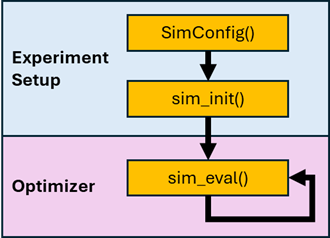
\includegraphics[width=0.35\textwidth]{sim_loops.png}
    \caption{High level overview of important simulation interfaces for setting up an experiment and evaluating fitness using an optimizer.}
    \label{fig:sim_loops}
\end{figure}


\begin{figure}
    \centering
    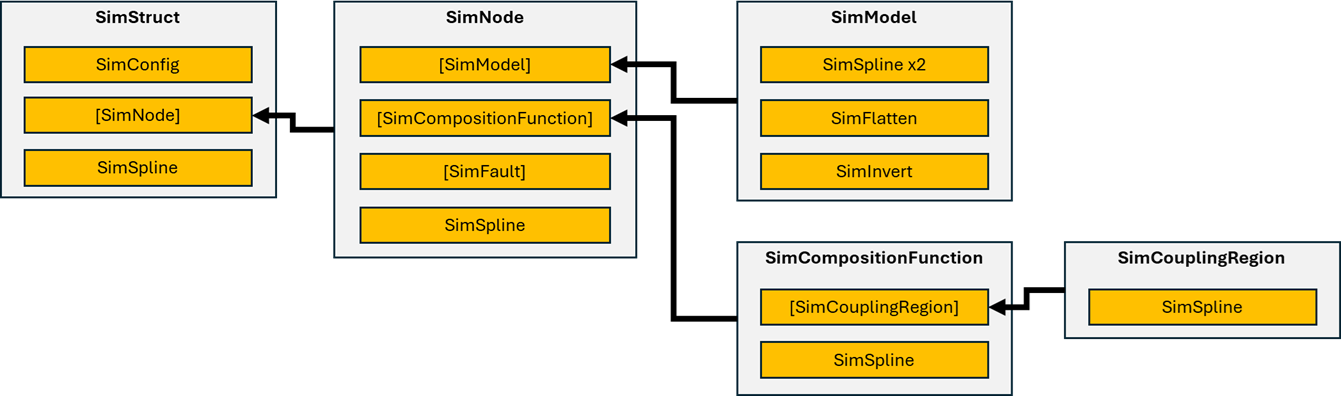
\includegraphics[width=1.0\textwidth]{sim_structs.png}
    \caption{Hierarchical relationship diagram of important simulation structures. Names in brackets indicate arrays. }
    \label{fig:sim_structs}
\end{figure}


The sim\_init function constructs the simulation using the provided configuration object. During simulation construction a log of the scenario features and configuration parameters is written to the filename provided in the logfile configuration parameter or the file "logfile.txt" by default (Req. 8). Additional debug figures can be created by enabling the save\_debug\_figs option. After the simulation is constructed, the number of design inputs required for evaluating the simulation scenario is stored in the num\_inputs simulation object parameter.

Scenario level randomization is controlled by seeding an Xoshiro random number stream from the Random package using the scenario seed configuration parameter (Req. 3, 48). This stream is used for constructing the simulation prior to execution (Req. 2). Run level randomization is controlled by seeding another Xoshiro random number stream using the noise seed configuration parameter plus the run iteration (Req. 3, 48).

A simulation run is performed by calling the sim\_eval function with the simulation object, the design parameters, the desired network path (Req. 13), and a fidelity level (Req. 17). This function reports a single value for the fitness score (Req. 5, 15) in the range [0, 1), with 1.0-$\epsilon$ being optimal, where $\epsilon$ is the minimum 64 bit floating point value (Req. 16). In the event of an infeasible solution, the fitness score is reported as NaN (Req. 6). An example simulation input array is provided in Figure \ref{fig:input_matrix}. Each input value is continuous in the range [0, 1). This example shows two nodes, each with five dimensions. Each node contains two composition functions, contain constraint pairs. Each composition function and each node have an additional scaling function input value. The first block of inputs are design values, and the last two inputs are used to determine the attempted network path. Details on all of these features are provided in the sections that follow.

\begin{figure}
    \centering
    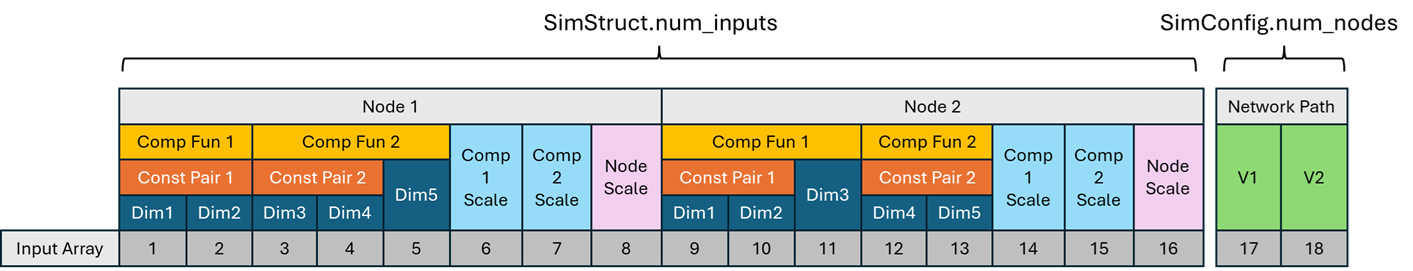
\includegraphics[width=0.96\textwidth]{input_matrix.png}
    \caption{Example input array with sixteen design inputs and two network path inputs. All values are continuous in the range [0, 1). Descriptions of the features in each column are provided in Section \ref{sec:simfeat}. }
    \label{fig:input_matrix}
\end{figure}

After each simulation run, the simulation object parameter num\_iterations contains the current run iteration and num\_function\_evals contains an updated cumulative number of function evaluations since the object was created (Req. 7). Due to dynamic and adversarial simulation features, each simulation run is coupled to the previous run and cannot be parallelized. The previous run score and number of iterations is stored as simulation state between runs. However, simulations with different starting noise seeds or starting input values can be parallelized to support niching optimization methods and validation of results.

The foundational element for creating landscapes in the simulation are spline basic functions. Spline basic functions are randomly generated splines using the scenario seed (Req. 2). The number of knots in the spline are randomly chosen using the min and max knots input parameters. Knots are added in series using the equation: $y[1] = rand() - rand(); y[i] = y[i-1] * knot\_feedback + rand() - rand()$. The knot\_feedback parameter is a value between 0 and 1 that determines how auto-correlated each knot is to the previous knot. When querying a spline function, the input and output ranges are clamped in the range [0.0, 1.0]. Spline basic functions are used throughout the simulation for creating governing, model, scaling, constraint, and adversarial functions as described in the following sections.


\section{Simulation Features}
\label{sec:simfeat}

\subsection{Governing Functions and Model Functions}

The governing functions and model functions are created using the spline basic function generator (Req. 22, 23).
The model response landscape is created by mapping design variable inputs to model function outputs through a governing function (Req. 24).
For example, a governing function $g(x)$ (Fig. \ref{fig:basic_eq_mdl_1_gov_fun}) is used to map input value x to model function $f(u)$ (Fig. \ref{fig:basic_eq_mdl_1_mdl_fun}) resulting in a multi-featured model response landscape $f(g(x))$ (Fig. \ref{fig:basic_eq_mdl_1_mdl_resp}).
Figure \ref{fig:landscape_mdl_19_mdl_resp} illustrates an example model response with many combined features: smooth, discontinuous, narrow and wide basins, shallow and deep basins, multi-modal, flattened, and non-linear (Req. 28). This example shows variable conditioning between the input and response (Req. 31), many potential optimal locations with values at 1.0 to support niching optimization methods (Req. 18), as well as multiple deceptive basins near 1.0 (Req. 29).
Flattening may occur when a governing or model function is clamped in the range [0, 1], however additional random flattening can be injected using the enable\_flattening configuration parameter (Fig. \ref{fig:flat_mdl_1_mdl_resp_flat}). Moreover, additional random discontinuity can be injected by randomly inverting regions using the enable\_inversion configuration parameter (Fig. \ref{fig:invert_mdl_1_mdl_resp_invert}).

\begin{figure}
	\centering
    \begin{minipage}[t]{0.47\textwidth}
        \centering
        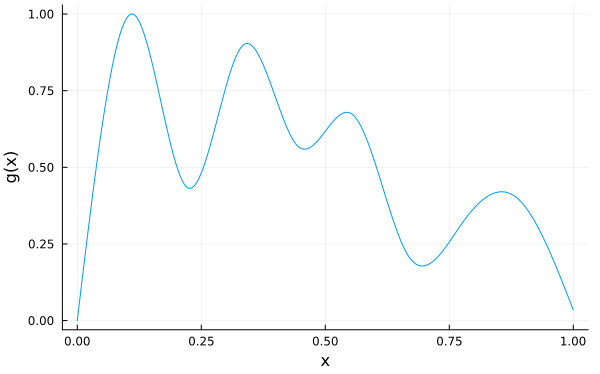
\includegraphics[width=0.97\textwidth]{basic_eq_mdl_1_gov_fun.png}
        \caption{Governing function created using a spline basic function.}
        \label{fig:basic_eq_mdl_1_gov_fun}
    \end{minipage}\hfill
    \begin{minipage}[t]{0.47\textwidth}
        \centering
        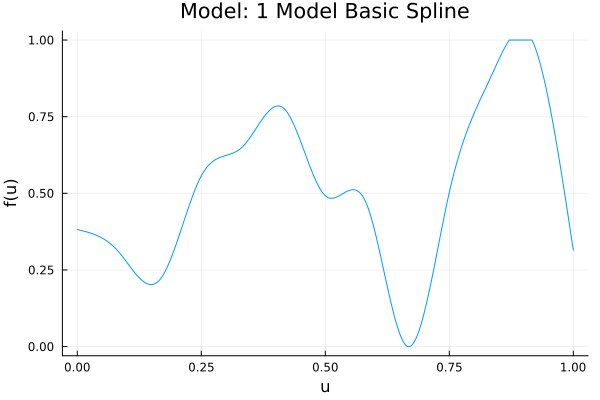
\includegraphics[width=0.97\textwidth]{basic_eq_mdl_1_mdl_fun.png}
        \caption{Model function created using a spline basic function.}
        \label{fig:basic_eq_mdl_1_mdl_fun}
    \end{minipage}
\end{figure}



\begin{figure}
	\centering
    \begin{minipage}[t]{0.47\textwidth}
        \centering
        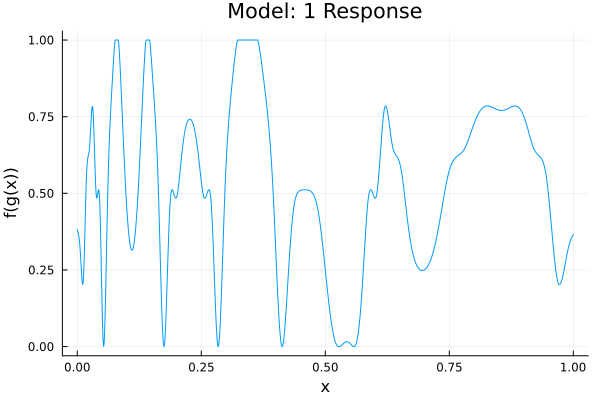
\includegraphics[width=0.97\textwidth]{basic_eq_mdl_1_mdl_resp.png}
        \caption{Model response landscape created by mapping design variable input to model function input through a governing function.}
        \label{fig:basic_eq_mdl_1_mdl_resp}
    \end{minipage}\hfill
    \begin{minipage}[t]{0.47\textwidth}
        \centering
        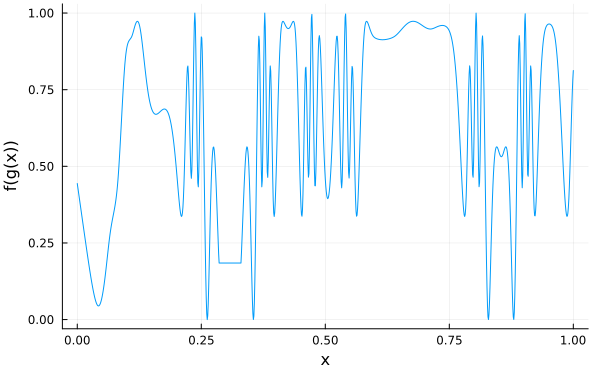
\includegraphics[width=0.97\textwidth]{landscape_mdl_19_mdl_resp.png}
        \caption{Example model response with many combined features: smooth, discontinuous, narrow and wide basins, shallow and deep basins, multi-modal, flattened, non-linear, and deceptive basins.}
        \label{fig:landscape_mdl_19_mdl_resp}
    \end{minipage}
\end{figure}



\begin{figure}
	\centering
    \begin{minipage}[t]{0.47\textwidth}
        \centering
        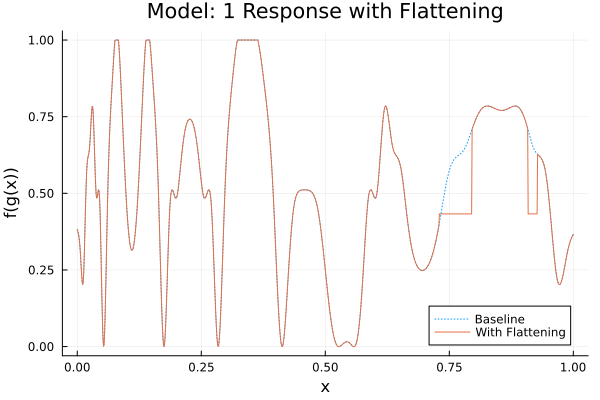
\includegraphics[width=0.97\textwidth]{flat_mdl_1_mdl_resp_flat.png}
        \caption{Example random flattening injected using the enable\_flattening configuration parameter.}
        \label{fig:flat_mdl_1_mdl_resp_flat}
    \end{minipage}\hfill
    \begin{minipage}[t]{0.47\textwidth}
        \centering
        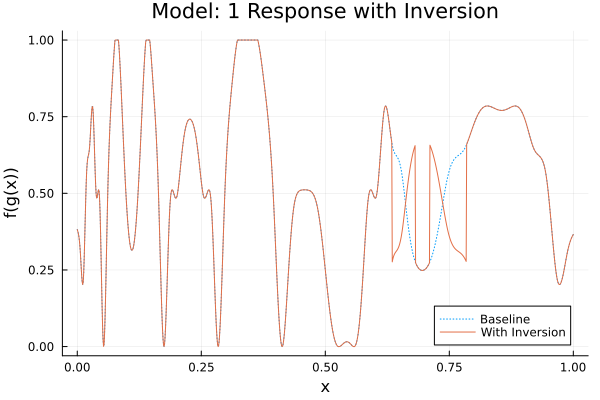
\includegraphics[width=0.97\textwidth]{invert_mdl_1_mdl_resp_invert.png}
        \caption{Example random discontinuity injected using the enable\_inversion configuration parameter.}
        \label{fig:invert_mdl_1_mdl_resp_invert}
    \end{minipage}
\end{figure}


\subsection{Composition Functions}

Composition functions are created by taking the weighted sum of model responses (Req. 25). The number of composition functions and the assignment of model functions to composition functions is random based on scenario seed and scaled by number of dimensions (Req. 14, 27). Model function weights are randomly chosen during scenario creation. Randomly assigning model functions to different composition functions creates a mixture of separable and non-separable inputs (Req. 12).

For each composition function, an additional input dimension is created for a scaling effect on the composition function response. This scaling function uses the spline basic function generator. When the simulation is evaluated, this scaling multiplier is applied to the composition function (Req. 30). For each node, an additional input dimension is created using the same process and applied as a scaling factor to the combination of composition functions. This results in D + C + 1 inputs per node, where D is the number of dimensions, C is the number of scale factors for composition functions, plus one for the final combined scaling factor function. The total fitness for each node is the weighted sum of each composition function at that node (Req. 38).

Figure \ref{fig:2d_const_3_1_base} illustrates an example composition landscape of the sum of two models. Many optimal locations at 1.0 are present to support niching optimization methods (Req. 18). An iso-optimal surface is created by scaling the composition response and inverting any portion that exceeds a value of 1.0. Figure \ref{fig:2d_const_3_1_iso} illustrates an iso-optimal surface that provides many disconnected iso-optimal regions (Req. 44) further facilitating niching optimization methods (Req. 18). Iso-optimal surfaces are scaled with the number of composition functions (Req. 45) with an additional global iso-optimal surface created for the overall node response (Req. 43).


\begin{figure}
	\centering
    \begin{minipage}[t]{0.47\textwidth}
        \centering
        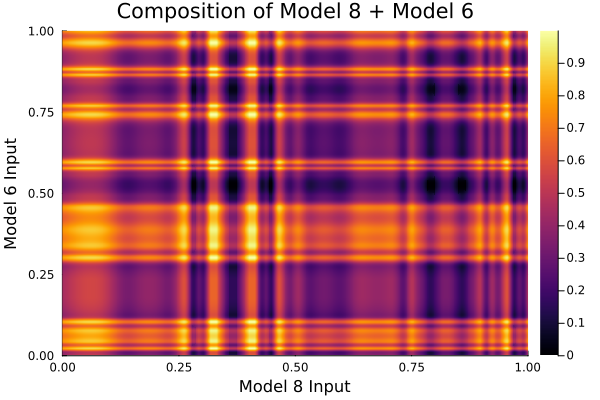
\includegraphics[width=0.97\textwidth]{2d_const_3_1_base.png}
        \caption{Example composition function response of two models.}
        \label{fig:2d_const_3_1_base}
    \end{minipage}\hfill
    \begin{minipage}[t]{0.47\textwidth}
        \centering
        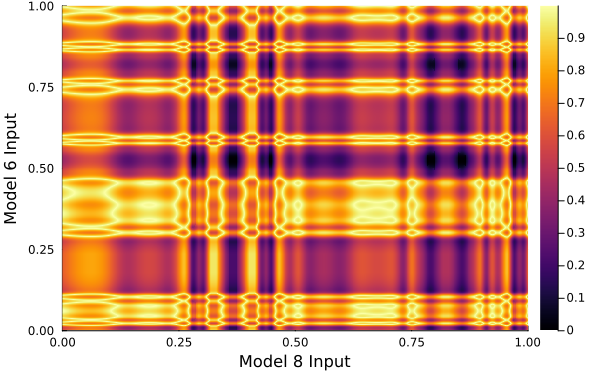
\includegraphics[width=0.97\textwidth]{2d_const_3_1_iso.png}
        \caption{Composition function response with added iso-optimal surface feature.}
        \label{fig:2d_const_3_1_iso}
    \end{minipage}
\end{figure}



\subsection{Skewing and Constraints}

During the creation of composition functions, pairs of dimensions are randomly coupled to create non-separability and non-axis alignment effects (Req. 12, 26). A skewing effect is created by randomly picking a skewing factor for each input. The first input is skewed as a function of the second input, then the second input is skewed as a function of the skewed first input. Skewing may be positive or negative and is controlled using the enable\_skewing and max\_skew\_magnitude configuration parameters. Figure \ref{fig:2d_const_3_1_iso_skew} illustrates skewing applied to the previous example. Skewed model inputs are wrapped in the range [0, 1] to remain valid and prevent regions of the solution landscape from becoming unreachable.

Feasibility constraints are created on coupled composition pairs using a constraint function. The constraint function is created using the spline basic function generator (Req. 32). One of the pair input values is selected as the constraint function input. Feasibility is determined by checking if the other pair input value is above or below (chosen at random for the constraint) of the spline response. The couple pair input values are transformed using their respective governing functions prior to evaluating the constraint function creating a varied feasibility landscape (Req. 33). Figure \ref{fig:2d_const_3_1_iso_skew_const} builds on the previous skewing example with additional infeasible regions shown in white (Req. 34). Constraints are applied to pairs of inputs resulting in separable and non-separable constraints when more than one constraint is present (Req. 35).

A couple margins are included to prevent a scenario in which there are no feasible optimal solutions. The first is an input margin controlled via the constraint\_input\_margin configuration parameter that requires the input variable enter the infeasible region by at least that amount before infeasibility is declared. The second margin is a small margin around optimal locations controlled via the constraint\_optimal\_margin configuration parameter. This margin results in small islands of optimal feasible solutions in Figure \ref{fig:2d_const_3_1_iso_skew_const}. A three-dimensional example is provided in Figure \ref{fig:compo_iso_3d}.


\begin{figure}
	\centering
    \begin{minipage}[t]{0.47\textwidth}
        \centering
        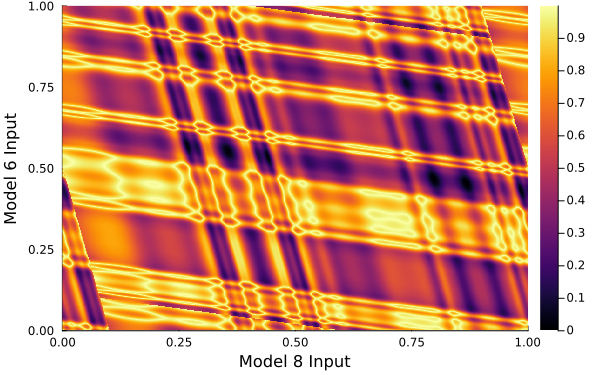
\includegraphics[width=0.97\textwidth]{2d_const_3_1_iso_skew.png}
        \caption{Composition function response with added wrapped skewing feature to create non-separability and non-axis alignment.}
        \label{fig:2d_const_3_1_iso_skew}
    \end{minipage}\hfill
    \begin{minipage}[t]{0.47\textwidth}
        \centering
        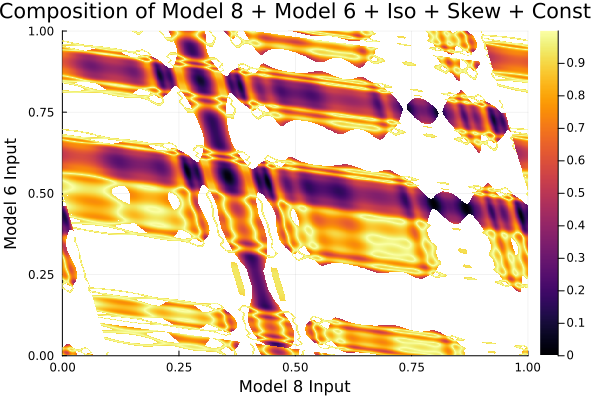
\includegraphics[width=0.97\textwidth]{2d_const_3_1_iso_skew_const.png}
        \caption{Composition function response with added feasibility constraint feature. White areas correspond to infeasible results.}
        \label{fig:2d_const_3_1_iso_skew_const}
    \end{minipage}
\end{figure}

\begin{figure}
	\centering
    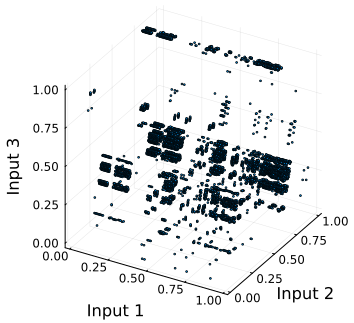
\includegraphics[width=0.6\textwidth]{compo_iso_3d.png}
    \caption{An example iso-optimal surface for a 3-Dimensional composition function with skewing and constraint features. All points displayed have a fitness of approximately 1.0.}
    \label{fig:compo_iso_3d}
\end{figure}


\subsection{Dynamic Features}

The simulation provides features for dynamically changing the scenario structure as a function of optimization iterations with the enable\_dynamic configuration option. During each call to sim\_eval(), the num\_iterations counter increments which affects continuous changes and discrete events. Continuous changes are created by through the use of a velocity parameter for each input dimension and generating function response (Fig. \ref{fig:test_dyn_model}). For a constant input value, each simulation iteration will cause the composition function and constraint landscapes to slowly change (Req. 56, 57). This feature is controlled using the enable\_dynamic\_spline, dyn\_model\_inp\_vel\_mag, and dyn\_model\_gen\_vel\_mag configuration parameters.

Multiple dynamic discrete events features are available (Req. 54). Each design input is assigned a random offset during scenario creation using the enable\_input\_shift option. If dynamic features are enabled, the enable\_dynamic\_input\_shift option will result in periodic jump shifts for each input offset. The magnitude and frequency of the shifts are controlled via the dyn\_input\_shift\_mag, input\_shift\_freq\_min, and dyn\_input\_shift\_freq\_max feature respectively. When the number of iterations reaches a randomly selected threshold between the min and max frequency (Req. 52) all inputs will be offset simultaneously resulting in a new bias in the design inputs. This will result in dynamic jumps in the composition function and constraint landscapes (Req. 58). Figure \ref{fig:test_dyn_input_shift} shows three input shifting events (indicated by black circles) across four-thousand simulation evaluations sweeping across a design input from zero to one.

Each design input is mapped to simulation models using a mapping vector, enabled using the enable\_input\_map option (Req. 51). If dynamic features are enabled as well as the enable\_dynamic\_input\_map option, then the mapping of design variables to models will randomly mutate at discrete events (Req. 58). Mutations occur between random pairs of inputs at a random simulation iteration chosen between the frequency ranges defined in the dyn\_input\_map\_freq\_min and dyn\_input\_map\_freq\_max configuration parameters. Figure \ref{fig:test_dyn_map} illustrates a dynamic input mapping change event at the 1000th simulation iteration while sweeping the input dimension from zero to one over two-thousand evaluations. Figure \ref{fig:test_dyn_map_spline} shows an example response of the combination of the continuous input velocity feature and the discrete input mapping change event.

Lastly, the simulation supports a dynamic discrete event feature to periodically mutate the simulation network when using more than one node (Req. 55). This feature is enabled using the enable\_dynamic\_network option. The frequency of the event is controlled using the dyn\_network\_map\_freq\_min and dyn\_network\_map\_freq\_max configuration parameters. The network mutation event swaps two nodes along the nominal path so that the majority of the path remains valid. However, random links between paths are regenerated from scratch at each event (Req. 49).


\begin{figure}
	\centering
    \begin{minipage}[t]{0.47\textwidth}
        \centering
        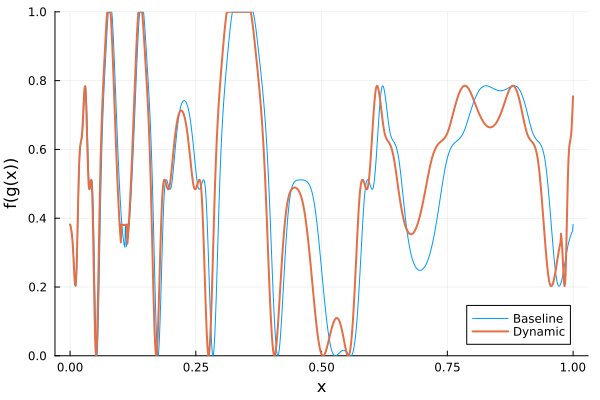
\includegraphics[width=0.97\textwidth]{test_dyn_model.png}
    \caption{Example model response showing continuous dynamic spline landscape change as a function of simulation iterations.}
    \label{fig:test_dyn_model}
    \end{minipage}\hfill
    \begin{minipage}[t]{0.47\textwidth}
        \centering
        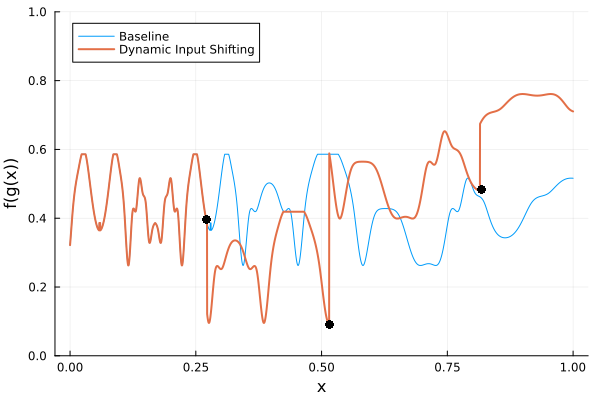
\includegraphics[width=0.97\textwidth]{test_dyn_input_shift.png}
    \caption{Example model response with discrete dynamic input shift biasing events as a function of simulation iterations.}
    \label{fig:test_dyn_input_shift}
    \end{minipage}
\end{figure}


\begin{figure}
	\centering
    \begin{minipage}[t]{0.47\textwidth}
        \centering
        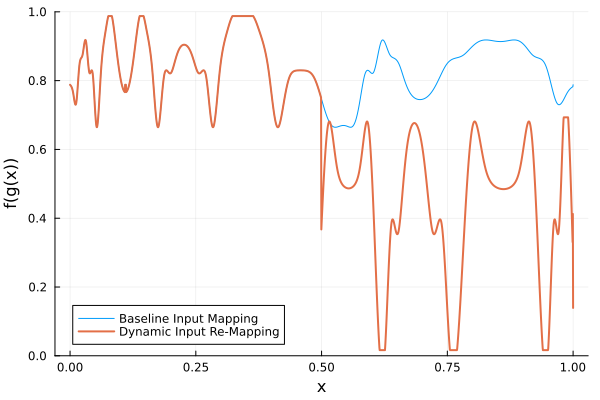
\includegraphics[width=0.97\textwidth]{test_dyn_map.png}
    \caption{Example model response with discrete design input re-mapping event as a function of simulation iterations.}
    \label{fig:test_dyn_map}
    \end{minipage}\hfill
    \begin{minipage}[t]{0.47\textwidth}
        \centering
        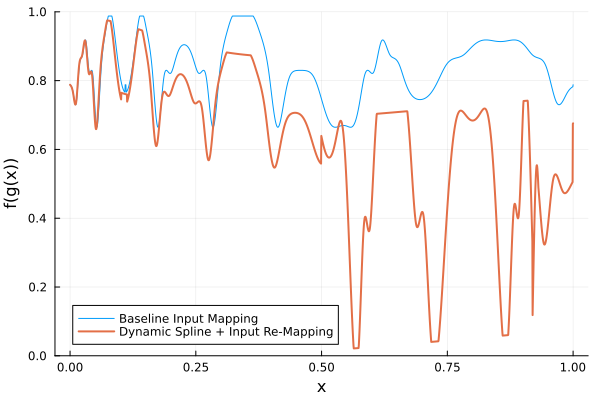
\includegraphics[width=0.97\textwidth]{test_dyn_map_spline.png}
    \caption{Example model response that combines a discrete input re-mapping event with continuous dynamic spline landscape changes as a function of simulation iterations.}
    \label{fig:test_dyn_map_spline}
    \end{minipage}
\end{figure}



\subsection{Stochastic Features}

The simulation provides a variety of stochastic features to challenge optimizers. Noise can be added to the design input values to create uncertainty into the generating functions (Req. 26). This is controlled via the enable\_input\_noise and input\_noise\_sigma configuration parameters. Because the uncertainty is created at the generating function inputs this results in uncertainty at constraint boundaries (Req. 50). Additionally, noise can be added to the model response outputs using the enable\_model\_noise and model\_noise\_sigma configuration parameters (Req. 47). Figures \ref{fig:comp2d_input_noise} and \ref{fig:comp2d_model_noise} illustrate these respective features.


\begin{figure}
	\centering
    \begin{minipage}[t]{0.47\textwidth}
        \centering
        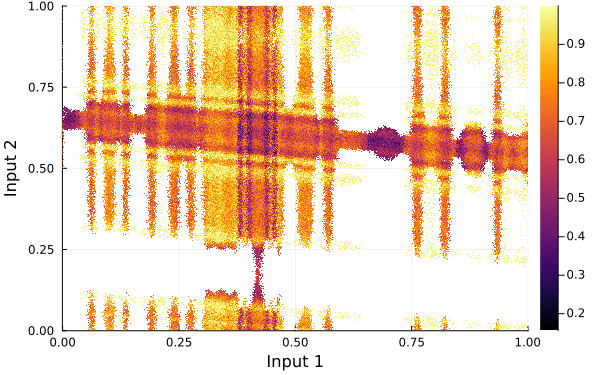
\includegraphics[width=0.97\textwidth]{comp2d_input_noise.png}
        \caption{Stochastic composition function response created by noise added to input dimensions.}
        \label{fig:comp2d_input_noise}
    \end{minipage}\hfill
    \begin{minipage}[t]{0.47\textwidth}
        \centering
        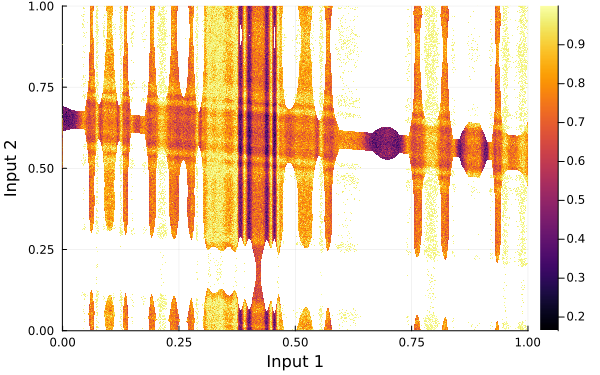
\includegraphics[width=0.97\textwidth]{comp2d_model_noise.png}
        \caption{Stochastic composition function response created by noise added to model responses.}
        \label{fig:comp2d_model_noise}
    \end{minipage}
\end{figure}



\subsection{Variable Model Fidelity}

When evaluating simulation fitness, the optimizer must include an integer parameter for model fidelity (Req. 17). This allows replicates to be performed when determining input and response uncertainty during simulation evaluation. The number of replicates is determined by raising the fidelity value to the power specified in the fidelity\_power configuration parameter, rounded to the nearest integer above zero. Figure \ref{fig:test_fidelity_var_1} provides an example in which a single design input value is provided while raising the fidelity input from one to ten across one-thousand simulation evaluations showing a convergence in fitness response. Figure \ref{fig:test_fidelity_var_2} illustrates this effect while sweeping the design input from zero to one while raising the fidelity from one to ten across one-thousand simulation evaluations.


\begin{figure}
	\centering
    \begin{minipage}[t]{0.47\textwidth}
        \centering
        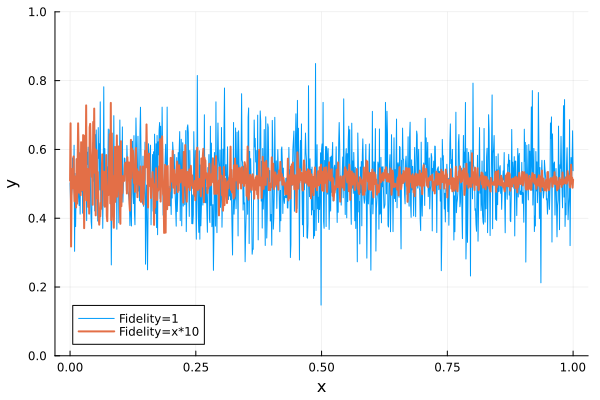
\includegraphics[width=0.97\textwidth]{test_fidelity_var_1.png}
        \caption{Demonstration of model fitness convergence by increasing model fidelity from one to ten.}
        \label{fig:test_fidelity_var_1}
    \end{minipage}\hfill
    \begin{minipage}[t]{0.47\textwidth}
        \centering
        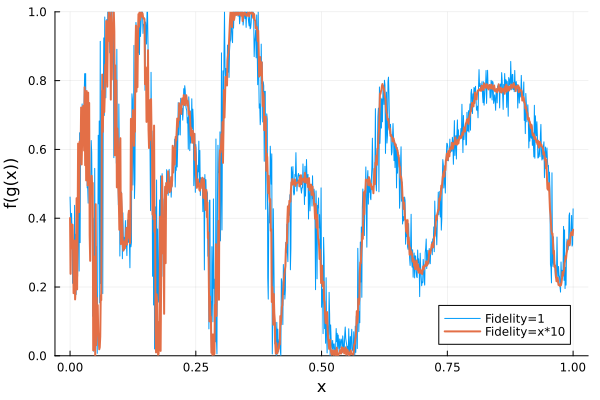
\includegraphics[width=0.97\textwidth]{test_fidelity_var_2.png}
        \caption{Example model response while increasing model fidelity from one to ten as design input variable x is increased from zero to one.}
        \label{fig:test_fidelity_var_2}
    \end{minipage}
\end{figure}


\subsection{Semi-Cooperative Features}

The simulation supports a variety of semi-cooperative features. These are features in which the simulation intentionally reports randomly incorrect results (Req. 65), to include feasibility or infeasibility (Req. 66), as well as fails to execute based on pre-determined fault injection thresholds (Req. 62). When the enable\_random\_fitness configuration option is enabled, the random\_fitness\_rate controls how often incorrect random fitness reports are returned from the simulation.

During scenario creation, some input dimensions are randomly selected to include fault injection with a corresponding failure threshold and magnitude. When a fault is present and the evaluated model response falls below the failure threshold the model response will be either degraded by scaling downward (Fig. \ref{fig:fault_mdl_5_mdl_resp_fault_degrade}) or will result in a simulation executive failure (Fig. \ref{fig:fault_mdl_8_mdl_resp_fault_029}) (Req. 61). In the event of an executive failure the simulation will report 0.0 for the fitness score and will provide no indication that a failure was triggered. Fault via degradation and fault via executive failure result in separable and non-separable failure regions (Req. 63). Figure \ref{fig:comp2d_inp_model_noise_faults} provides an example composition of two dimensions, input noise, model noise, random failure and infeasibility, as well as large black executive failure regions.


\begin{figure}
	\centering
    \begin{minipage}[t]{0.47\textwidth}
        \centering
        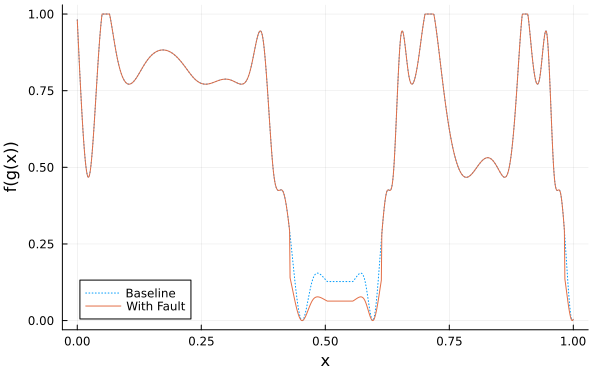
\includegraphics[width=0.97\textwidth]{fault_mdl_5_mdl_resp_fault_degrade.png}
	\caption{Example model fault resulting in degraded response.}
	\label{fig:fault_mdl_5_mdl_resp_fault_degrade}
    \end{minipage}\hfill
    \begin{minipage}[t]{0.47\textwidth}
        \centering
        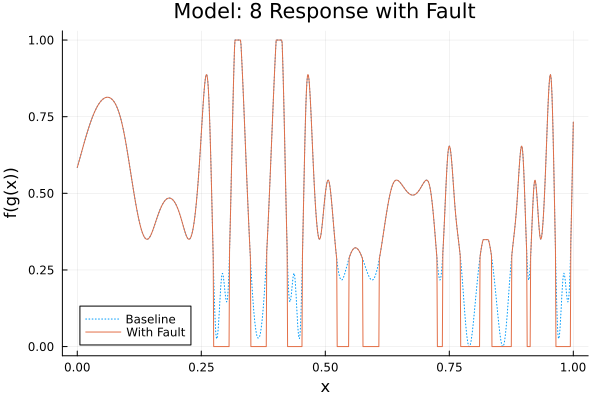
\includegraphics[width=0.97\textwidth]{fault_mdl_8_mdl_resp_fault_0.29.png}
	\caption{Example model complete failure triggered at locations where the model response falls below 0.29.}
	\label{fig:fault_mdl_8_mdl_resp_fault_029}
    \end{minipage}
\end{figure}



\subsection{Adversarial Features}

The simulation creates an adversarial optimization environment as a function of the weighted history of fitness results, enabled using the enable\_adversarial configuration option (Req. 20). The simulation object contains an adversarial\_fitness state value that is continually updated each simulation evaluation by blending in the current iterations fitness value. The weighting of the blending is controlled via the adversarial\_feedback parameter, resulting in a temporal memory of fitness with greater weight on the most recent solutions. The magnitude of the adversarial\_fitness state value determines the scaling of adversarial features. This value is combined with a spline basic function to create non-linear artifacts in the scaling using the equation $x * (1 + s(s(x) - 0.5) * 0.5)$ where x is the adversarial\_fitness value in the range [0,1] and s(x) is the adversarial spline basic function evaluated at x (Figure \ref{fig:out_adversarial_fun}).

The first method for adversarial feedback is by non-linear movement in the fitness landscape. if adversarial features are enabled in addition to the enable\_adversarial\_offset parameter, then each design input variables will be injected with a random bias scaled by the adversarial\_offset\_mag configuration parameter. This results in stronger movement in optimal basins if the recent fitness evaluations were near optimal. This effect is illustrated in Figure \ref{fig:test_adv_offset_l2r} and \ref{fig:test_adv_offset_r2l} by sweeping the design input from zero to one and then one to zero respectively. Different movements in the fitness landscapes are created based on recent fitness evaluations independent of what design inputs were used in the evaluations (Req. 59).

The second method for adversarial feedback is by scaling the frequency of random incorrect results, random failure and random infeasibility events, and input and model uncertainty (Req. 60). This is created by enabling the enable\_adversarial\_incorrect, enable\_adversarial\_failure, and enable\_adversarial\_noise configuration options respectively. The adversarial\_incorrect\_factor, adversarial\_failure\_factor, and adversarial\_noise\_factor configuration parameters increase the random\_fitness\_rate, random\_fault\_rate, and random\_infeasible\_rate frequencies by a multiple of (1.0 + factor * adversarial scaling) respectively. Figure \ref{fig:test_adv_fail} illustrates additional random failure events when the input value is near optimal around zero. Figure \ref{fig:test_adv_noise} illustrates the scaling in the uncertainty distribution by showing larger variance around the fitness solution as optimality is approached and equivalent uncertainty for fitness values near zero (Req. 53).



\begin{figure}
	\centering
    \begin{minipage}[t]{0.47\textwidth}
        \centering
        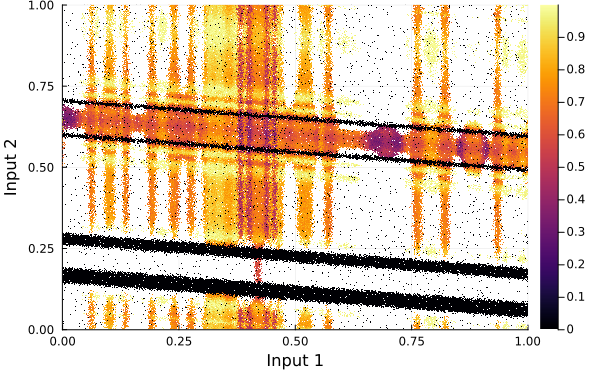
\includegraphics[width=0.97\textwidth]{comp2d_inp_model_noise_faults.png}
	\caption{Example combining a two-dimensional composition function with input and model uncertainty, random failures and infeasibility reports, as well as executive failure regions.}
	\label{fig:comp2d_inp_model_noise_faults}
    \end{minipage}\hfill
    \begin{minipage}[t]{0.47\textwidth}
        \centering
        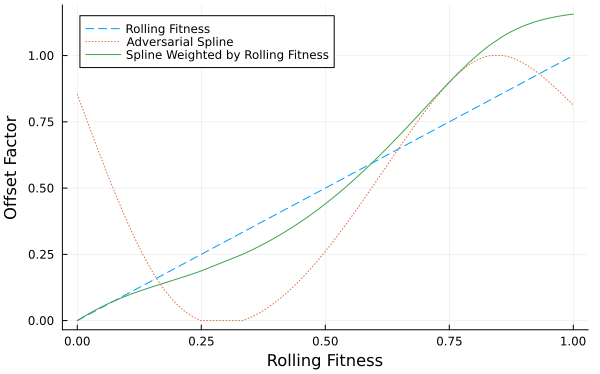
\includegraphics[width=0.97\textwidth]{out_adversarial_fun.png}
	\caption{Construction of adversarial scaling factor by weighted sum of spline basic function and rolling fitness score.}
	\label{fig:out_adversarial_fun}
    \end{minipage}
\end{figure}

\begin{figure}
	\centering
    \begin{minipage}[t]{0.47\textwidth}
        \centering
        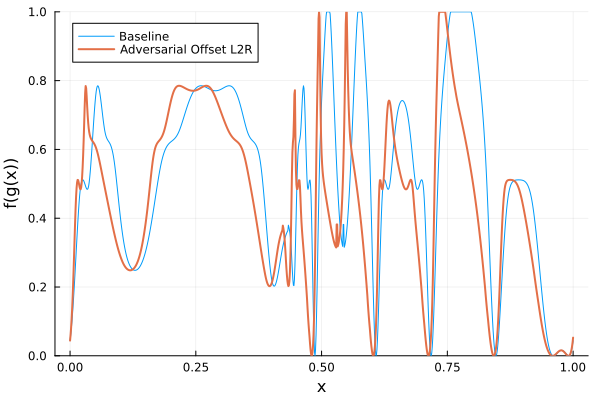
\includegraphics[width=0.97\textwidth]{test_adv_offset_l2r.png}
	\caption{Application of adversarial scaling factor to model input bias while scanning input dimension x from zero to one (left to right) illustrating the temporal relationship in adversarial fitness memory.}
	\label{fig:test_adv_offset_l2r}
    \end{minipage}\hfill
    \begin{minipage}[t]{0.47\textwidth}
        \centering
        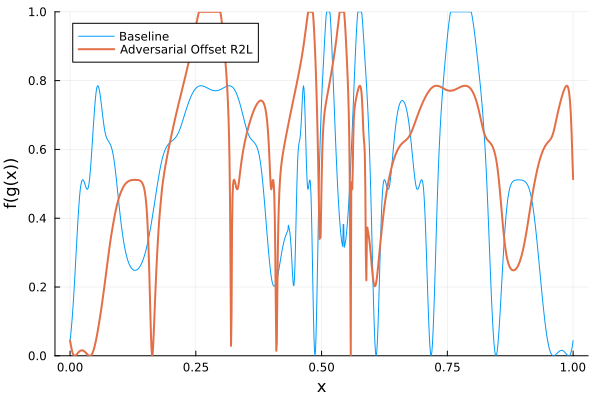
\includegraphics[width=0.97\textwidth]{test_adv_offset_r2l.png}
	\caption{Application of adversarial scaling factor to model input bias while scanning input dimension x from one to zero (right to left) illustrating the temporal relationship in adversarial fitness memory.}
	\label{fig:test_adv_offset_r2l}
    \end{minipage}
\end{figure}

\begin{figure}
	\centering
    \begin{minipage}[t]{0.47\textwidth}
        \centering
        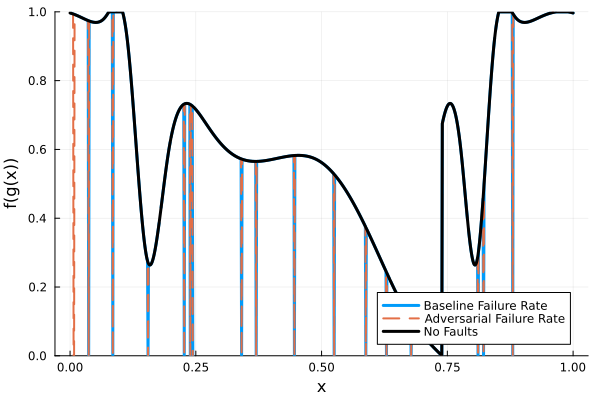
\includegraphics[width=0.97\textwidth]{test_adv_fail.png}
	\caption{Example showing an elevation in random failure events due to adversarial response when the rolling fitness score is near optimal.}
	\label{fig:test_adv_fail}
    \end{minipage}\hfill
    \begin{minipage}[t]{0.47\textwidth}
        \centering
        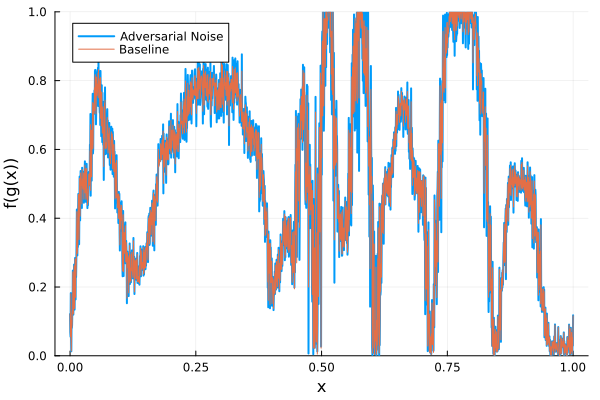
\includegraphics[width=0.97\textwidth]{test_adv_noise.png}
	\caption{Example showing an elevation in input and model noise due to adversarial response when the rolling fitness score is near optimal.}
	\label{fig:test_adv_noise}
    \end{minipage}
\end{figure}


\subsection{Network Pathfinding}

The simulation capabilities discussed thus far apply to individual nodes. These nodes can be included in a scalable directed network where the number of nodes in the network is set in the simulation configuration object. Each node is visited in turn using an optimizer provided path array to the sim\_eval() function (Req. 36). When the simulation is initialized, a nominal network path is created using a random permutation of the node numbers. Each node in the permutation has a valid exit linking it to the next node in the permutation creating a linear directed graph with one path through all of the nodes. Additional random directed links are created based on the node\_random\_connection\_freq configuration parameter, as illustrated in Figure \ref{fig:network} (Req. 49).

\begin{figure}
    \centering
    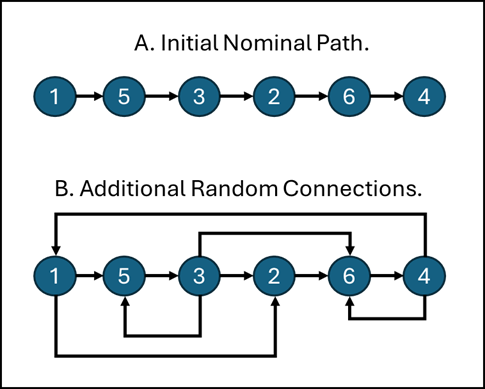
\includegraphics[width=0.4\textwidth]{network.png}
    \caption{A: An example directed network single nominal path with six nodes. B: Random directed links added to the nominal path.}
    \label{fig:network}
\end{figure}

The total fitness for the simulation evaluation is a weighted combination of the fitness function of each node that is visited (Req. 39). Node weighting is randomly set upon initialization and then additionally linearly scaled as a function of index in the nominal path such that successfully reaching later nodes tends to have a higher impact on the overall fitness (Req. 41). The combination of continuous node design inputs with discrete node index pathfinding results in combined continuous and mixed-integer problems (Req. 11).

The simulation can enforce that certain nodes in the network are visited or else the run fails (Req. 42). This is enabled using the enable\_node\_required\_visits option with number of required node visits determined using the node\_visit\_required\_rate parameter. The rate parameter is multiplied by the number of nodes to set the first N nodes in the nominal path as required for visitation or else the simulation will return a failure fitness of 0.0. Lastly, if the optimizer provides an invalid path through the network, to include visiting a node multiple times, the simulation will stop crawling the network (Req. 40). At this point the simulation can return the current fitness or return a failure fitness of 0.0 if the option enable\_fail\_on\_bad\_path is set (Req. 64).


\section{Experimentation Method}

This section describes a series of experiments for tuning the configuration parameters and comparing optimization performance using the Crucible Simulation. Depending on the experiment, different optimization strategies were used. These included the Evolutionary Centers Algorithm (ECA), Particle Swarm Optimization (PSO), and Simulated Annealing (SA) optimizers from the Metaheuristics.jl package \cite{mejia-de-dios_metaheuristics_2022} using a population size of one-hundred for each, as well as Random Search (RND) as described below. This population size was used for each algorithm for consistency and chosen because one-hundred was used in the Metaheuristics.jl documentation examples for PSO and SA. The fitness tolerance was set to 1e-5, and the function call limit and number of iterations was set to ten-thousand. All other options were defaults, no hyper-parameter optimization was performed.

During each simulation iteration, the designated optimizer provides an array of values to a callback function with the length of the array equal to the number of simulation inputs (sim.num\_inputs) plus the number of nodes (sim.config.num\_nodes). The first portion of the inputs pass through as design variables. The node inputs are sorted by value and the resulting index order is provided as the desired network path thus allowing a continuous input space for a mixed-integer optimization problem. The simulation fitness is evaluated using the design inputs, network path, and fidelity level 1 (lowest). If an infeasible solution NaN is returned the score is set to 0.0. Next, the number of simulation iterations is decremented and the adversarial feedback is temporarily set to 1.0 before running the simulation again with the best known inputs thus far and saving the regression fitness. This allows the experiment to measure the quality of the best known inputs at each iteration without affecting dynamic and adversarial features. If the current iteration score is higher than this regression fitness then the current iteration inputs are set as the new best known inputs. After each iteration, the best known fitness is appended to a result array.

Each experiment treatment runs ten replicates of thirty scenario seeds for ten-thousand iterations. This results in three-million fitness scores per treatment in the result array. This array is used for post-processing to find the 50th and 90th percentile best fitness scores, $F_{50}$ and $F_{90}$ respectively, for each treatment. In the event that the ECA, PSO, or SA optimizers stop before ten-thousand iterations due to convergence, the experiment continues to run until the iteration limit while storing the updated fitness at the best known input location. When dynamic features are enabled this could result in lower performance if an optimizer returns earlier than the requested number of iterations.

When Random Search (RND) is used, all design variables and node inputs are chosen from a random distribution in the range [0, 1) using the Xoshiro generator. The random number seed used by all optimizers starts at zero at the beginning of the treatment and increments by one after each replicate resulting in three-hundred total seeds per treatment.


\subsection{Experiment 0. Configuration Parameter Tuning}
\label{configparams}

Prior to running the performance comparison experiments, the simulation configuration parameters were tuned. As with the comparison experiments, ten replicates of thirty scenario seeds for ten-thousand iterations were used during each tuning cycle. Parameters were tuned using only the RND optimizer to allow features to have an observable impact without overly burdening or improving performance. The descriptions of parameters with setpoint justification is provided below in Table \ref{tbl:sim-config}.

Before tuning, the following inputs were explicitly set as described in Table \ref{tbl:sim-config}: model noise sigma, fidelity power, flattening rate, inversion rate, random fault rate, random infeasible rate, random fitness rate, constraint input margin, constraint optimal margin, min knots, max knots, min scale knots, max scale knots, min constraint knots, max constraint knots, max skew magnitude, knot feedback, adversarial noise factor, adversarial incorrect factor, adversarial feedback, min adversarial knots, max adversarial knots, dyn input map freq min, dyn input map freq max, dyn network map freq min, dyn network map freq max, dyn input shift freq min, dyn input shift freq max, node visit required freq, and node random connection freq.

Next, feature configuration parameters were tuned by running the designated experiment size using scenarios with five nodes of five dimensions. For each configuration parameter, a baseline $F_{50}$ score was calculated with no effect, then bisection search was used to find a parameter setpoint that reached a specific $F_{50}$ performance delta. This was chosen to balance the effect of different features on overall performance. After tuning, the parameters place the 90th percentile fitness ($F_{90}$) score just above 0.0 when all features were enabled in the four-dimension-four-node scenarios of Experiment 3, thereby providing wide comparative illustration of the compounding effect of each feature on optimizer performance.

The first parameter tuned was the iso-optimal threshold. As the threshold is reduce from 1.0, the iso-optimal surface area grows making solutions easier to find. Bisection search was used to improve the $F_{50}$ score to place it at 0.70. For the remaining parameters, the baseline score included the following enabled features: input mapping, input shifting, composition function scaling, node total fitness scaling, spline flattening, spline inversion, model noise, spline couple pair skewing, and node visitation requirements. The following parameters were tuned to create a -0.02 $\Delta F_{50}$: input noise sigma, dyn model inp vel mag, dyn model gov vel mag, dyn inp shift, adversarial offset mag, and adversarial failure factor. Adversarial features were tuned with only iso-optimal enabled to improve performance so that the effect is more visible. Lastly, due to the interaction between fault threshold and fault degradation rate, fault max thresh was first tuned to create a -0.015 $\Delta F_{50}$ with degradation rate set to 0.0. Then fault degradation rate was increased to create a +0.005 $\Delta F_{50}$, this way the combination of inputs resulted in an overall delta of only -0.01.


\begingroup

\newcolumntype{C}[1]{>{\centering\arraybackslash}p{#1}}

\begin{longtable}{| p{0.28\linewidth} | C{0.08\linewidth} | p{0.26\linewidth} | p{0.26\linewidth} | }

\caption{Simulation Configuration Parameters.}\\

\hline
\textbf{Parameter} & \textbf{Default} & \textbf{Description} & \textbf{Justification} \\ \hline
\endfirsthead

\hline
\textbf{Parameter} & \textbf{Default} & \textbf{Description} & \textbf{Justification} \\ \hline
\endhead

\multicolumn{4}{|l|}{\cellcolor{lightgray}\textbf{Scenario Options}} \\ \hline
structure\_seed & 0 & Sim structure RNG seed & Zero initialized \\ \hline
noise\_seed & 0 & Run variation RNG seed & Zero initialized \\ \hline
num\_dimensions & 1 & Number of dimensions at each node & Minimum valid value \\ \hline
num\_nodes & 1 & Number of nodes in the network & Minimum valid value \\ \hline

\multicolumn{4}{|l|}{ } \\ \hline
\multicolumn{4}{|l|}{\cellcolor{lightgray}\textbf{Feature Parameters}} \\ \hline
input\_noise\_sigma & 0.0016 & Variation in decision variables & Achieve $\Delta F_{50}$ of -0.02 during tuning \\ \hline
model\_noise\_sigma & 0.01 & Variation in model outputs & Limit 3 $\sigma$ spread to 0.06 \\ \hline
fidelity\_power & 1.5 & Power of variable fidelity noise reduction & Desired convergence at fidelity level 10 \\ \hline
flattening\_rate & 0.3 & Probability of enabling flattening on splines & Support landscape variation \\ \hline
inversion\_rate & 0.3 & Probability of enabling inversion on splines & Support landscape variation \\ \hline
random\_fault\_rate & 0.02 & Probability of returning a random fault result & To achieve 2\% on average \\ \hline
random\_infeasible\_rate & 0.02 & Probability of returning a random infeasible result & To achieve 2\% on average \\ \hline
random\_fitness\_rate & 0.02 & Probability of returning a random result & To achieve 2\% on average \\ \hline
fault\_degredation\_rate & 0.37 & Probability of degradation instead of fault & Achieve $\Delta F_{50}$ of -0.010 during tuning \\ \hline
fault\_max\_thresh & 0.77 & Upper limit to fault threshold & Achieve $\Delta F_{50}$ of -0.015 during tuning \\ \hline
constraint\_input\_margin & 0.05 & Distance input must enter constraint to return infeasible & Large enough to prevent no feasible result \\ \hline
constraint\_optimal\_margin & 0.05 & Distance away from optimal before applying constraint & Large enough to prevent no optimal result \\ \hline
min\_knots & 10 & Minimum knots for governing and model splines & Support landscape variation \\ \hline
max\_knots & 20 & Maximum knots for governing and model splines & Support landscape variation \\ \hline
min\_scale\_knots & 5 & Minimum knots for scaling splines & Achieve non-linear scaling \\ \hline
max\_scale\_knots & 10 & Maximum knots for scaling splines & Achieve non-linear scaling \\ \hline
min\_constraint\_knots & 10 & Minimum knots for constraint splines & Support landscape variation \\ \hline
max\_constraint\_knots & 20 & Maximum knots for constraint splines & Support landscape variation \\ \hline
max\_skew\_magnitude & 0.3 & Maximum skew ratio for coupled model outputs & Meaningful reduction in axis alignment \\ \hline
knot\_feedback & 0.5 & Temporal feedback in spline basic functions & Support landscape variation \\ \hline
adversarial\_offset\_mag & 0.14 & Magnitude of input shifting during adversarial feedback & Achieve $\Delta F_{50}$ of -0.02 during tuning \\ \hline
adversarial\_noise\_factor & 3 & Magnitude of noise amplification during adversarial feedback & Limit 3 $\sigma$ spread to 0.06 \\ \hline
adversarial\_failure\_factor & 0.33 & Additional failure rate during adversarial feedback & Achieve $\Delta F_{50}$ of -0.02 during tuning \\ \hline
adversarial\_incorrect\_factor & 3 & Magnitude of random result amplification during adversarial feedback & Achieve 6\% when near optimal \\ \hline
adversarial\_feedback & 0.8 & Temporal feedback in fitness score for adversarial features & Demonstrated temporal memory \\ \hline
min\_adversarial\_knots & 5 & Minimum knots for adversarial feature spline & Support non-linear spline landscape \\ \hline
max\_adversarial\_knots & 10 & Maximum knots for adversarial feature spline & Support non-linear spline landscape \\ \hline
dyn\_model\_inp\_vel\_mag & 0.0077 & Maximum input offset velocity magnitude per 1000 sim iterations & Achieve $\Delta F_{50}$ of -0.02 during tuning \\ \hline
dyn\_model\_gov\_vel\_mag & 0.0077 & Maximum governing offset velocity magnitude per 1000 sim iterations & Achieve $\Delta F_{50}$ of -0.02 during tuning \\ \hline
dyn\_input\_map\_freq\_min & 1050 & Minimum iterations before input re-mapping event & Achieve 6 to 9 events per 10k iterations \\ \hline
dyn\_input\_map\_freq\_max & 1600 & Maximum iterations before input re-mapping event & Achieve 6 to 9 events per 10k iterations \\ \hline
dyn\_network\_map\_freq\_min & 1050 & Minimum iterations before network re-mapping event & Achieve 6 to 9 events per 10k iterations \\ \hline
dyn\_network\_map\_freq\_max & 1600 & Maximum iterations before network re-mapping event & Achieve 6 to 9 events per 10k iterations \\ \hline
dyn\_input\_shift\_freq\_min & 1450 & Minimum iterations before input offset shift event & Achieve 3 to 5 events per 10k iterations \\ \hline
dyn\_input\_shift\_freq\_max & 1700 & Maximum iterations before input offset shift event & Achieve 3 to 5 events per 10k iterations \\ \hline
dyn\_input\_shift\_mag & 0.0071 & Maximum offset during input shift event & Achieve $\Delta F_{50}$ of -0.02 during tuning \\ \hline
node\_visit\_required\_freq & 0.1 & Frequency of selecting a node for required visitation & Minimally demonstrated effect \\ \hline
node\_random\_connection\_freq & 0.2 & Frequency of adding extra random node connections & Support non-linear node networks \\ \hline

\multicolumn{4}{|l|}{ } \\ \hline
\multicolumn{4}{|l|}{\cellcolor{lightgray}\textbf{Feature Enablement}} \\ \hline
enable\_input\_map & TRUE & Enable the input mapping feature & Max difficulty by default \\ \hline
enable\_input\_shift & TRUE & Enable the input shifting feature & Max difficulty by default \\ \hline
enable\_input\_noise & TRUE & Enable the input noise feature & Max difficulty by default \\ \hline
enable\_model\_noise & TRUE & Enable the model noise feature & Max difficulty by default \\ \hline
enable\_adversarial & TRUE & Enable adversarial features & Max difficulty by default \\ \hline
enable\_adversarial\_noise & TRUE & Enable adversarial noise feature & Max difficulty by default \\ \hline
enable\_adversarial\_offset & TRUE & Enable adversarial offset feature & Max difficulty by default \\ \hline
enable\_adversarial\_failure & TRUE & Enable adversarial failure feature & Max difficulty by default \\ \hline
enable\_adversarial\_incorrect & TRUE & Enable adversarial incorrect feature & Max difficulty by default \\ \hline
enable\_dynamic & TRUE & Enable dynamic feature & Max difficulty by default \\ \hline
enable\_dynamic\_spline & TRUE & Enable dynamic spline feature & Max difficulty by default \\ \hline
enable\_dynamic\_input\_map & TRUE & Enable dynamic input map feature & Max difficulty by default \\ \hline
enable\_dynamic\_input\_shift & TRUE & Enable dynamic input shift feature & Max difficulty by default \\ \hline
enable\_dynamic\_network & TRUE & Enable dynamic network feature & Max difficulty by default \\ \hline
enable\_constraints & TRUE & Enable feasibility constraints feature & Max difficulty by default \\ \hline
enable\_flattening & TRUE & Enable spline flattening feature & Max difficulty by default \\ \hline
enable\_faults & TRUE & Enable fault features & Max difficulty by default \\ \hline
enable\_inversion & TRUE & Enable spline inversion feature & Max difficulty by default \\ \hline
enable\_iso\_optimal & TRUE & Enable iso optimal surface feature & Max difficulty by default \\ \hline
enable\_skewing & TRUE & Enable coupled response skewing feature & Max difficulty by default \\ \hline
enable\_comp\_scale\_inputs & TRUE & Enable composition function scaling inputs & Max difficulty by default \\ \hline
enable\_total\_scale\_input & TRUE & Enable total node fitness scaling inputs & Max difficulty by default \\ \hline
enable\_random\_fitness & TRUE & Enable random fitness result feature & Max difficulty by default \\ \hline
enable\_node\_required\_visits & TRUE & Enable node visitation required feature & Max difficulty by default \\ \hline
enable\_fail\_on\_bad\_path & TRUE & Enable executive failure on invalid network path & Max difficulty by default \\ \hline
quiet\_init & FALSE & Print simulation construction log to console & Reduce console output by default \\ \hline
save\_debug\_figs & FALSE & Save simulation construction debug figures & Not needed for normal runs


\label{tbl:sim-config} \\ \hline


\end{longtable}

\endgroup


\subsection{Experiment 1. Optimizer Comparison by Varying Dimension Quantity }

The first experiment was performed to compare the impact of raising the number of dimensions on a single node while using different optimization algorithms with all features off and all features on. The full-factorial experiment design is captured in Table \ref{tbl:exp1-doe} for a total of forty treatments. The standard setup of ten replicates of thirty scenario seeds for ten-thousand iterations was performed for each experiment treatment resulting in one-hundred-and-twenty-million runs. Results from this experiment are illustrated and described in Section \ref{sec:results-1}.


%--------------------------------------------------------------------------------------------
%--------------------------------------------------------------------------------------------
\begin{table}[H]
	\centering
	\caption{Experiment 1 Design}
	\label{tbl:exp1-doe}
	\newcolumntype{C}[1]{>{\centering\arraybackslash}p{#1}}
	\begin{tabular}{| p{0.12\linewidth} | C{0.08\linewidth} | C{0.08\linewidth} | C{0.08\linewidth} | C{0.08\linewidth} | }
	\hline
	\textbf{Factors} & \multicolumn{4}{c|}{\textbf{Levels}} \\ \hline
	Features & \multicolumn{2}{c|}{All Off} & \multicolumn{2}{c|}{All On} \\ \hline
	Algorithm & RND & ECA & PSO & SA \\ \hline
	Dimensions & \multicolumn{4}{@{}c@{}|}{\hspace*{\fill} 1 \hspace*{\fill}\vrule\hspace*{\fill} 3 \hspace*{\fill}\vrule\hspace*{\fill} 5 \hspace*{\fill}\vrule\hspace*{\fill} 10 \hspace*{\fill}\vrule\hspace*{\fill} 20 \hspace*{\fill}} \\ \hline
	Nodes & \multicolumn{4}{c|}{1} \\ \hline
	\end{tabular}
\end{table}


\subsection{Experiment 2. Optimizer Comparison by Varying Node Quantity }

The results from Experiment 1 were used to down-select the optimization algorithms to RND and ECA only based on their comparable good performance in Experiment 1 with all features enabled. This second experiment varied the number of nodes from one to five while keeping the number of dimensions fixed at four and compare the performance for all features on and all features off. Four dimensions were selected so that scenarios could be generated with multiple two composition functions of coupled pairs with constraints, thereby allowing all features to participate in impacting performance, while not being overly burdensome. The full-factorial experiment design is captured in Table \ref{tbl:exp2-doe} for a total of twenty treatments. Using the standard replicate and scenario setup resulted in sixty-million runs. Results from this experiment are illustrated and described in Section \ref{sec:results-2}.


%--------------------------------------------------------------------------------------------
%--------------------------------------------------------------------------------------------

\begin{table}[H]
	\centering
	\caption{Experiment 2 Design}
	\label{tbl:exp2-doe}	
	\newcolumntype{C}[1]{>{\centering\arraybackslash}p{#1}}
	\begin{tabular}{| p{0.12\linewidth} | C{0.16\linewidth} | C{0.16\linewidth} | }
	\hline
	\textbf{Factors} & \multicolumn{2}{c|}{\textbf{Levels}} \\ \hline
	Features & All Off & All On \\ \hline
	Algorithm & RND & ECA \\ \hline
	Dimensions & \multicolumn{2}{c|}{4} \\ \hline
	Nodes & \multicolumn{2}{@{}c@{}|}{\hspace*{\fill} 1 \hspace*{\fill}\vrule\hspace*{\fill} 2 \hspace*{\fill}\vrule\hspace*{\fill} 3 \hspace*{\fill}\vrule\hspace*{\fill} 4 \hspace*{\fill}\vrule\hspace*{\fill} 5 \hspace*{\fill}} \\ \hline
	\end{tabular}
\end{table}


\subsection{Experiment 3. Optimizer Comparison Across Features }

The results from Experiment 1 and 2 were used to select four nodes with four dimensions as the network configuration for Experiment 3. This provided a challenging test case for illustrating the effects of individual features. The experiment was perform in two phases. The first phase performed the standard set of three million iterations (ten replicates, thirty scenarios, with ten-thousand iterations each) while enabling features in isolation to compare their individual impact against a baseline with no features enabled. The second phase performed the standard three million iterations while enabling features in series to compare their cumulative impact against a baseline with no features enabled. Both phases were performed using RND and ECA optimization for comparison. The full-factorial design is provided in Table \ref{tbl:exp3-doe}, resulting in three-hundred-and-twelve-million runs. Results from this experiment are illustrated and described in Section \ref{sec:results-3}.



%--------------------------------------------------------------------------------------------
%--------------------------------------------------------------------------------------------

\begin{table}[H]
	\centering
	\caption{Experiment 3 Design}
	\label{tbl:exp3-doe}	
	\newcolumntype{C}[1]{>{\centering\arraybackslash}p{#1}}
	\begin{tabular}{| p{0.12\linewidth} | C{0.16\linewidth} | C{0.16\linewidth} | }
	\hline
	\textbf{Factors} & \multicolumn{2}{c|}{\textbf{Levels}} \\ \hline
	Features & Individual & Cumulative \\ \hline
	Algorithm & RND & ECA \\ \hline
	Dimensions & \multicolumn{2}{c|}{4} \\ \hline
	Nodes & \multicolumn{2}{c|}{4} \\ \hline
	\end{tabular}
\end{table}





\section{Experiment Results}

The following sections describe and illustrate performance comparisons across the experiment designs.

\subsection{Experiment 1. Optimizer Comparison by Varying Dimension Quantity }
\label{sec:results-1}

Table \ref{tbl:exp1} provides $F_{50}$ and $F_{90}$ scores for RND, ECA, PSO, and SA optimizers for Experiment 1. Scores show consistent degradation in performance as the number of dimensions is increased from one to twenty. CDF curves are provided to illustrate the full performance distributions across the parametric dimension sweep. Each curve shows the distribution of fitness scores for the best known inputs across three-million iterations. Better optimization performance is indicated by curves being more to the right with 1.0 fitness being optimal.

CDF Figures \ref{fig:test_exp_1_compare_rnd}, \ref{fig:test_exp_1_compare_eca}, \ref{fig:test_exp_1_compare_pso}, and \ref{fig:test_exp_1_compare_sa} show the performance sensitivity to dimension for RND, ECA, PSO, and SA respectively will all features off. ECA, PSO, and SA dominate RND performance with all features off. ECA and PSO are nearly equivalent with PSO outperforming at the higher dimensions. PSO and SA are equivalent for one dimension, however SA dominates all others for higher dimensions tested.

CDF Figures \ref{fig:test_exp_1b_compare_rnd}, \ref{fig:test_exp_1b_compare_eca}, \ref{fig:test_exp_1b_compare_pso}, and \ref{fig:test_exp_1b_compare_sa} show the performance sensitivity to dimension for RND, ECA, PSO, and SA respectively will all features on. These plots illustrate the drastic drop in performance by including all features. Contrary to the first set with all features off, PSO and SA perform markedly worse than RND and ECA with all features on. Interestingly, while ECA dominates PSO and SA, it only performs marginally better than RND for each dimension.


%--------------------------------------------------------------------------------------------
%--------------------------------------------------------------------------------------------
%--------------------------------------------------------------------------------------------


\begin{table}[H]
	\centering
	\caption{Experiment 1 Fitness Results for Adding Dimensions Across Four Optimizers}
	\label{tbl:exp1}
	\newcolumntype{C}[1]{>{\centering\arraybackslash}p{#1}}
	\begin{tabular}{| C{0.12\linewidth} | C{0.077\linewidth} | C{0.077\linewidth} | C{0.077\linewidth} | C{0.077\linewidth} | C{0.077\linewidth} | C{0.077\linewidth} | C{0.077\linewidth} | C{0.077\linewidth} | }
	\hline
	& \multicolumn{2}{c|}{RND} & \multicolumn{2}{c|}{ECA} & \multicolumn{2}{c|}{PSO} & \multicolumn{2}{c|}{SA} \\ \hline
    \textbf{Dimensions} & \textbf{$F_{50}$} & \textbf{$F_{90}$} & \textbf{$F_{50}$} & \textbf{$F_{90}$} & \textbf{$F_{50}$} & \textbf{$F_{90}$} & \textbf{$F_{50}$} & \textbf{$F_{90}$} \\ \hline

\multicolumn{9}{|l|}{\cellcolor{lightgray}\textbf{All Features OFF}} \\ \hline
1 & 1.000 & 1.000 & 1.000 & 1.000 & 1.000 & 1.000 & 1.000 & 1.000 \\ \hline
3 & 0.985 & 0.999 & 0.997 & 1.000 & 0.992 & 1.000 & 1.000 & 1.000 \\ \hline
5 & 0.929 & 0.970 & 0.962 & 0.991 & 0.950 & 0.990 & 1.000 & 1.000 \\ \hline
10 & 0.853 & 0.902 & 0.885 & 0.932 & 0.893 & 0.953 & 0.997 & 1.000 \\ \hline
20 & 0.766 & 0.832 & 0.796 & 0.859 & 0.820 & 0.885 & 0.984 & 1.000 \\ \hline

\multicolumn{9}{|l|}{ } \\ \hline
\multicolumn{9}{|l|}{\cellcolor{lightgray}\textbf{All Features ON}} \\ \hline
1 & 0.616 & 0.903 & 0.641 & 0.922 & 0.277 & 0.775 & 0.324 & 0.738 \\ \hline
3 & 0.508 & 0.785 & 0.524 & 0.805 & 0.178 & 0.611 & 0.229 & 0.629 \\ \hline
5 & 0.374 & 0.650 & 0.403 & 0.672 & 0.059 & 0.464 & 0.103 & 0.456 \\ \hline
10 & 0.099 & 0.405 & 0.103 & 0.415 & 0.000 & 0.185 & 0.000 & 0.199 \\ \hline
20 & 0.000 & 0.000 & 0.000 & 0.008 & 0.000 & 0.000 & 0.000 & 0.000 \\ \hline
	\end{tabular}
\end{table}



\begin{figure}
	\centering
    \begin{minipage}[t]{0.47\textwidth}
        \centering
        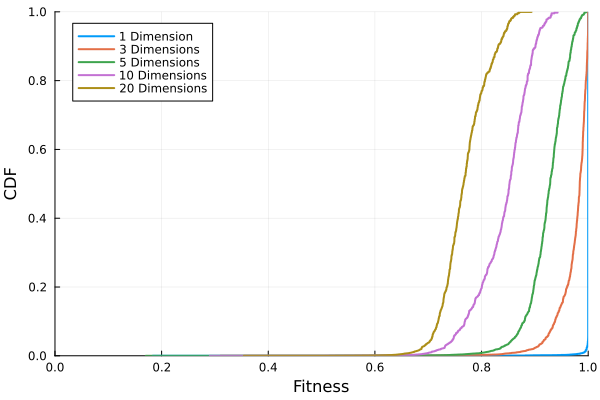
\includegraphics[width=0.97\textwidth]{test_exp_1_compare_rnd.png}
	\caption{Experiment 1 CDF curves of fitness for best inputs using the RND optimizer and all features off.}
	\label{fig:test_exp_1_compare_rnd}
    \end{minipage}\hfill
    \begin{minipage}[t]{0.47\textwidth}
        \centering
        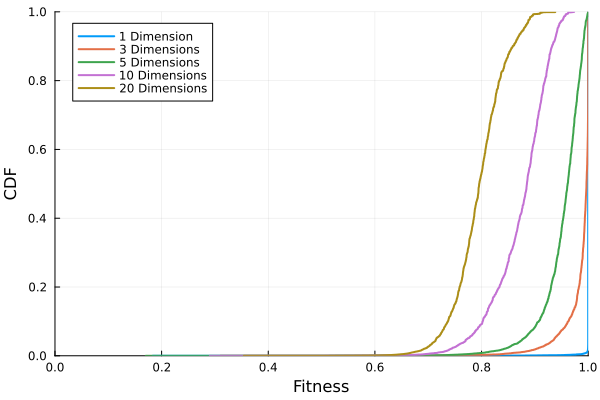
\includegraphics[width=0.97\textwidth]{test_exp_1_compare_eca.png}
	\caption{Experiment 1 CDF curves of fitness for best inputs using the ECA optimizer and all features off.}
	\label{fig:test_exp_1_compare_eca}
    \end{minipage}
\end{figure}


\begin{figure}
	\centering
    \begin{minipage}[t]{0.47\textwidth}
        \centering
        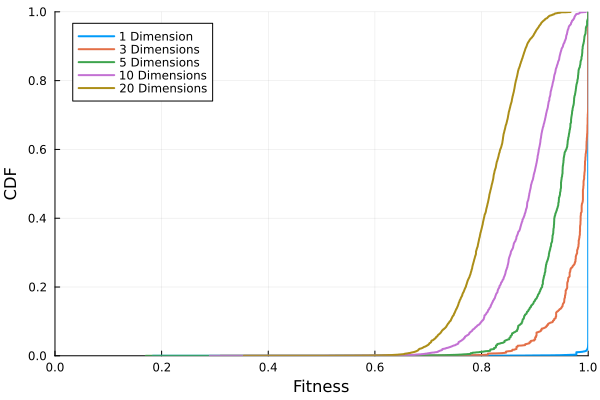
\includegraphics[width=0.97\textwidth]{test_exp_1_compare_pso.png}
	\caption{Experiment 1 CDF curves of fitness for best inputs using the PSO optimizer and all features off.}
	\label{fig:test_exp_1_compare_pso}
    \end{minipage}\hfill
    \begin{minipage}[t]{0.47\textwidth}
        \centering
        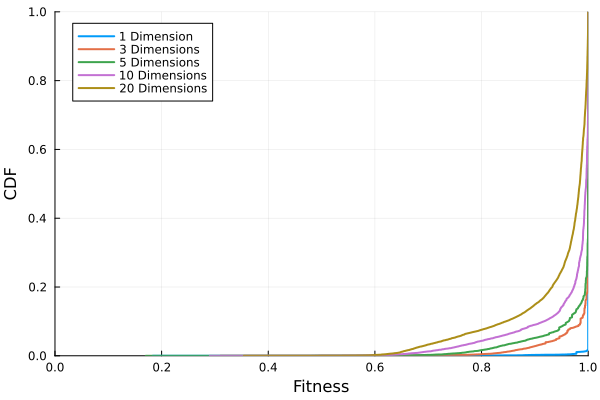
\includegraphics[width=0.97\textwidth]{test_exp_1_compare_sa.png}
	\caption{Experiment 1 CDF curves of fitness for best inputs using the SA optimizer and all features off.}
	\label{fig:test_exp_1_compare_sa}
    \end{minipage}
\end{figure}


\begin{figure}
	\centering
    \begin{minipage}[t]{0.47\textwidth}
        \centering
        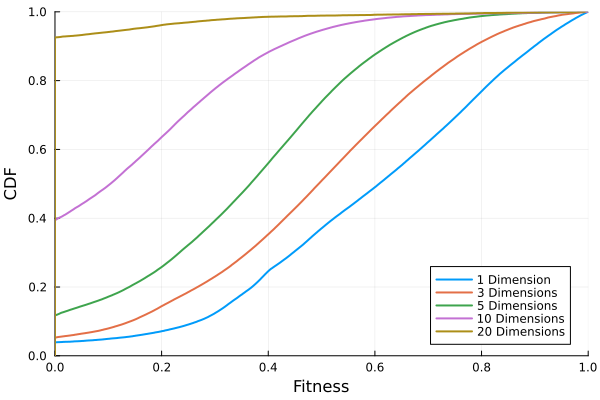
\includegraphics[width=0.97\textwidth]{test_exp_1b_compare_rnd.png}
	\caption{Experiment 1 CDF curves of fitness for best inputs using the RND optimizer and all features on.}
	\label{fig:test_exp_1b_compare_rnd}
    \end{minipage}\hfill
    \begin{minipage}[t]{0.47\textwidth}
        \centering
        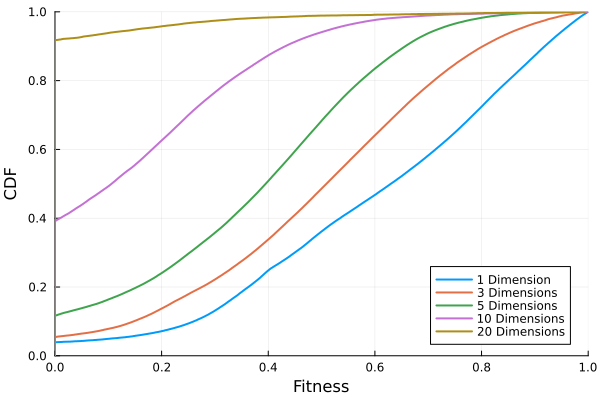
\includegraphics[width=0.97\textwidth]{test_exp_1b_compare_eca.png}
	\caption{Experiment 1 CDF curves of fitness for best inputs using the ECA optimizer and all features on.}
	\label{fig:test_exp_1b_compare_eca}
    \end{minipage}
\end{figure}



\begin{figure}
	\centering
    \begin{minipage}[t]{0.47\textwidth}
        \centering
        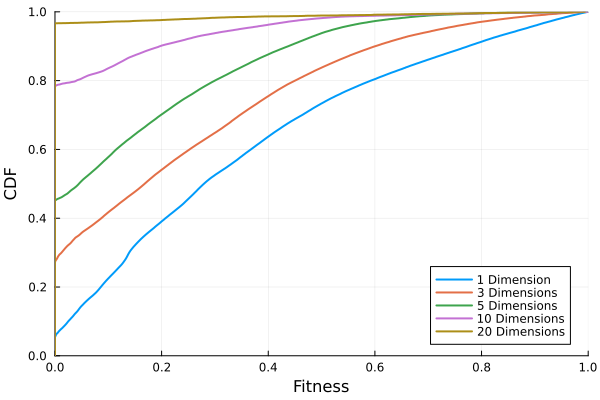
\includegraphics[width=0.97\textwidth]{test_exp_1b_compare_pso.png}
	\caption{Experiment 1 CDF curves of fitness for best inputs using the PSO optimizer and all features on.}
	\label{fig:test_exp_1b_compare_pso}
    \end{minipage}\hfill
    \begin{minipage}[t]{0.47\textwidth}
        \centering
        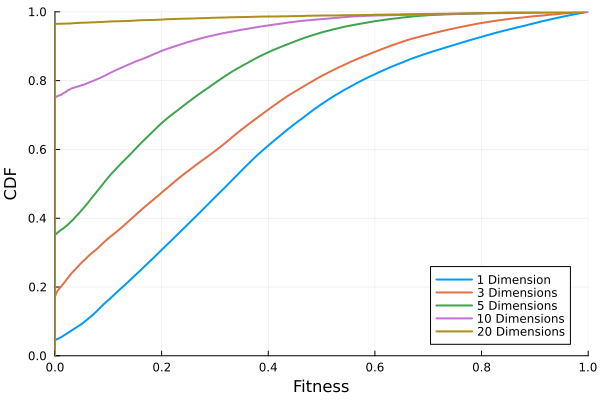
\includegraphics[width=0.97\textwidth]{test_exp_1b_compare_sa.png}
	\caption{Experiment 1 CDF curves of fitness for best inputs using the SA optimizer and all features on.}
	\label{fig:test_exp_1b_compare_sa}
    \end{minipage}
\end{figure}


\subsection{Experiment 2. Optimizer Comparison by Varying Node Quantity }
\label{sec:results-2}

Due to the strong performance of ECA in Experiment 1, it was chosen for comparing against RND for Experiment 2. Table \ref{tbl:exp2} provides $F_{50}$ and $F_{90}$ scores for RND and ECA optimizers while parametrically sweeping the number of nodes. CDF curves illustrate the distribution of fitness scores for the best known inputs across three-million iterations using the same method as Experiment 1.

CDF Figures \ref{fig:test_exp_2_compare_4dim_rnd}, \ref{fig:test_exp_2_compare_4dim_eca} show the performance sensitivity to node quantity for RND and ECA respectively will all features off. ECA shows marginally better performance than RND for a single node, however the improvement is much greater when more nodes are included in the network.

CDF Figures \ref{fig:test_exp_2b_compare_4dim_rnd}, \ref{fig:test_exp_2b_compare_4dim_eca} show the performance sensitivity to node quantity for RND and ECA respectively will all features on. Interestingly, ECA only shows marginally better performance than RND across all node combinations. Both RND and ECA have an $F_{90}$ score just above 0.0 at 0.033 and 0.023 respectively for four nodes. Both optimizers result in a 0.0 $F_{90}$ score for five nodes with four dimensions.


%--------------------------------------------------------------------------------------------
%--------------------------------------------------------------------------------------------
%--------------------------------------------------------------------------------------------


\begin{table}[H]
	\centering
	\caption{Experiment 2 Fitness Results for Adding Nodes with Four Dimensions}
	\label{tbl:exp2}	
	\newcolumntype{C}[1]{>{\centering\arraybackslash}p{#1}}
	\begin{tabular}{| C{0.11\linewidth} | C{0.11\linewidth} | C{0.11\linewidth} | C{0.11\linewidth} | C{0.11\linewidth} | }
	\hline
	 & \multicolumn{2}{c|}{RND} & \multicolumn{2}{c|}{ECA} \\ \hline
\textbf{Nodes} & \textbf{$F_{50}$} & \textbf{$F_{90}$} & \textbf{$F_{50}$} & \textbf{$F_{90}$} \\ \hline


\multicolumn{5}{|l|}{\cellcolor{lightgray}\textbf{All Features OFF}} \\ \hline
1 & 0.964 & 0.988 & 0.984 & 0.999 \\ \hline
2 & 0.866 & 0.930 & 0.911 & 0.959 \\ \hline
3 & 0.788 & 0.869 & 0.854 & 0.914 \\ \hline
4 & 0.724 & 0.798 & 0.800 & 0.872 \\ \hline
5 & 0.664 & 0.742 & 0.749 & 0.819 \\ \hline

\multicolumn{5}{|l|}{ } \\ \hline
\multicolumn{5}{|l|}{\cellcolor{lightgray}\textbf{All Features ON}} \\ \hline
1 & 0.470 & 0.725 & 0.491 & 0.749 \\ \hline
2 & 0.232 & 0.476 & 0.244 & 0.507 \\ \hline
3 & 0.000 & 0.271 & 0.000 & 0.252 \\ \hline
4 & 0.000 & 0.033 & 0.000 & 0.023 \\ \hline
5 & 0.000 & 0.000 & 0.000 & 0.000 \\ \hline
	\end{tabular}
\end{table}



\begin{figure}
	\centering
    \begin{minipage}[t]{0.47\textwidth}
        \centering
        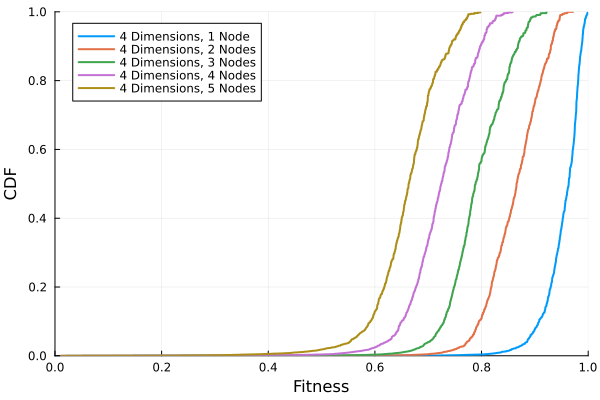
\includegraphics[width=0.97\textwidth]{test_exp_2_compare_4dim_rnd.png}
	\caption{Experiment 2 CDF curves of fitness for best inputs using the RND optimizer and all features off.}
	\label{fig:test_exp_2_compare_4dim_rnd}
    \end{minipage}\hfill
    \begin{minipage}[t]{0.47\textwidth}
        \centering
        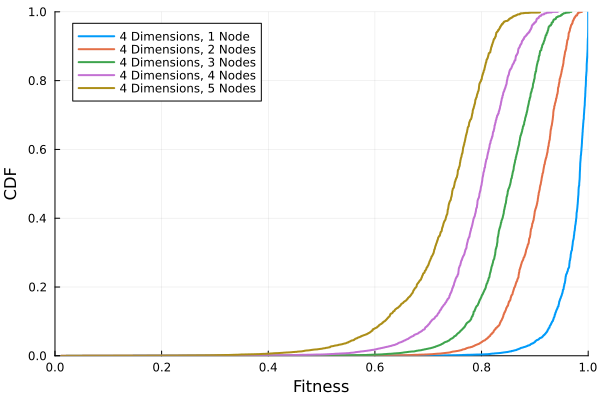
\includegraphics[width=0.97\textwidth]{test_exp_2_compare_4dim_eca.png}
	\caption{Experiment 2 CDF curves of fitness for best inputs using the ECA optimizer and all features off.}
	\label{fig:test_exp_2_compare_4dim_eca}
    \end{minipage}
\end{figure}



\begin{figure}
	\centering
    \begin{minipage}[t]{0.47\textwidth}
        \centering
        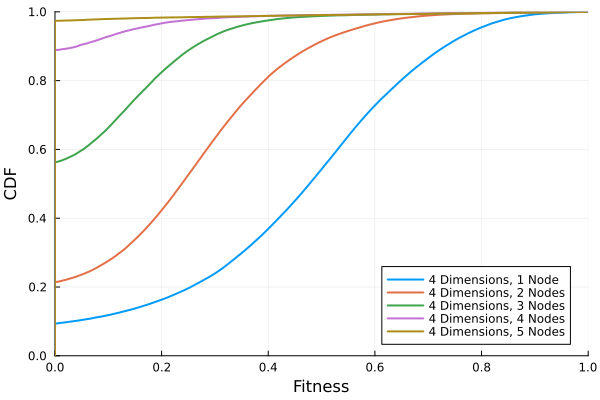
\includegraphics[width=0.97\textwidth]{test_exp_2b_compare_4dim_rnd.png}
	\caption{Experiment 2 CDF curves of fitness for best inputs using the RND optimizer and all features on.}
	\label{fig:test_exp_2b_compare_4dim_rnd}
    \end{minipage}\hfill
    \begin{minipage}[t]{0.47\textwidth}
        \centering
        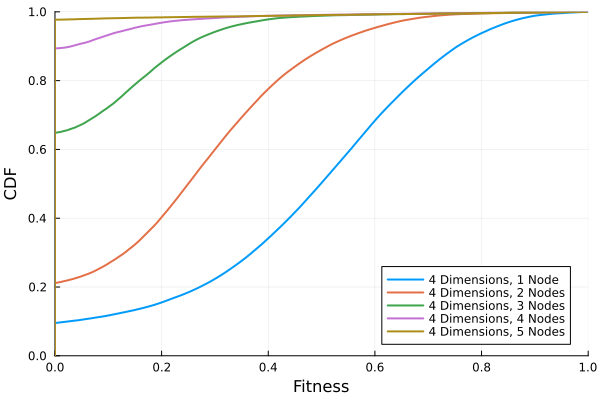
\includegraphics[width=0.97\textwidth]{test_exp_2b_compare_4dim_eca.png}
	\caption{Experiment 2 CDF curves of fitness for best inputs using the ECA optimizer and all features on.}
	\label{fig:test_exp_2b_compare_4dim_eca}
    \end{minipage}
\end{figure}


\subsection{Experiment 3. Optimizer Comparison Across Features }
\label{sec:results-3}

Experiment 3 builds upon the results from Experiments 1 and 2 to compare the performance of the RND and ECA optimizers while enabling features individually and in series. This experiment uses four nodes with four dimensions each to provide a challenging scenario without overburdening performance while supporting evaluation of the relative and compound impact of features. When all features are enabled the $F_{90}$ score for RND and ECA are just above 0.0. As with the previous experiments, each treatment includes the standard ten replicates of thirty scenarios with ten-thousand iterations each for a total of three-million iterations per treatment. Likewise, each of the CDF curves below represent the fitness score for the best known inputs across the three-million iterations. Due to simulation runtime and the number of features, pairwise sensitivity testing was not performed to quantify the impact of feature interactions.

\subsubsection{Impact of Individual Features}

Results for enabling individual features are provided in Table \ref{tbl:exp3-parallel} with Figures \ref{fig:test_exp_3_parallel_rnd} and \ref{fig:test_exp_3_parallel_eca} showing results for RND and ECA respectively. The first line in Table \ref{tbl:exp3-parallel} represents "baseline" performance, or performance with no features enabled other than composition functions with spline basic equations and network mapping logic. Each simulation feature is then enabled in isolation with the resulting $\Delta F_{50}$ and $\Delta F_{90}$ scores being the change in performance from baseline, thus representing the impact for enabling that feature. Individual delta scores are also provided in bar chart form in Figures \ref{fig:test_exp_3_parallel_f50} and \ref{fig:test_exp_3_parallel_f90} for $\Delta F_{50}$ and $\Delta F_{90}$ respectively.

The first important response is the positive score shift due to enabling the iso-optimal surface feature. This result is expected as it creates many large non-convex continuous and disconnected regions with an optimal score of 1.0 as opposed to considerably fewer small optimal islands. Enabling input noise adds uncertainty to the decision variables resulting in uncertainty propagation through the simulation calculations resulting in approximately -0.01 performance drop. The next series of features provide negligible performance difference and are primarily used to create landscape variation, non-separability, and add uncertainty to the output: model noise, input shift, input map, flattening, inversion, and skewing.

Enabling the feasibility constraint feature results in a large drop in performance of around -0.11. While constraints do not make the iso-optimal surface infeasible, they do drastically reduce the surface of feasible non-optimal solutions resulting in NaN being returned by the simulation if any input of the inputs result in an infeasible solution. Next, the composition function scaling and node total scaling inputs create a large drop in performance between -0.09 and -0.21. These enable the input decision variables that evaluate the scaling splines, effectively increasing the dimensionality of the problem space. Enabling faults shows meaningful but not extreme drop in performance of around -0.03 due to now including model fitness degradation and simulation executive failures.

Enabling dynamic features show no change in performance as expected due to sub-features not being enabled. Dynamic splines, input mapping, and input shifting each result in approximately -0.025 performance drop as expected from configuration parameter tuning. Dynamic network events results in larger movements for $F_{50}$ than $F_{90}$ by a magnitude of approximately three for a drop in $F_{50}$ of around -0.05 to -0.10.

Next, enabling adversarial features shows no change in performance as expected due to sub-features not being enabled, following the same pattern as for dynamic features. Enabling elevated adversarial noise to model outputs shows negligible overall delta as expected due to the lower average performance for four nodes with four dimensions as well as the noise being Gaussian. Next, the adversarial offset, failure, and incorrect features result in higher, but not extreme performance degradation of around -0.04 as expected from parameter tuning. However, the impact is noticeably larger for ECA than for RND. Lastly, the bad path failure and random fitness provide negligible overall delta in isolation.


%--------------------------------------------------------------------------------------------
%--------------------------------------------------------------------------------------------
%--------------------------------------------------------------------------------------------


\begin{table}[H]
	\centering
	\caption{Experiment 3 Fitness Sensitivity for Individual Features}
	\label{tbl:exp3-parallel}
	\newcolumntype{C}[1]{>{\centering\arraybackslash}p{#1}}
	\begin{tabular}{| p{0.2\linewidth} | C{0.12\linewidth} | C{0.12\linewidth} | C{0.12\linewidth} | C{0.12\linewidth} | C{0.12\linewidth} | }
	\hline
	 & \multicolumn{2}{c|}{RND} & \multicolumn{2}{c|}{ECA} \\ \hline
\textbf{Features} & \textbf{$\Delta F_{50}$} & \textbf{$\Delta F_{90}$} & \textbf{$\Delta F_{50}$} & \textbf{$\Delta F_{90}$} \\ \hline


baseline & 0.723 & 0.797 & 0.799 & 0.871 \\ \hline
iso\_optimal & +0.052 & +0.047 & +0.051 & +0.040 \\ \hline
input\_noise & -0.007 & -0.003 & -0.012 & -0.011 \\ \hline
model\_noise & 0.000 & +0.001 & -0.002 & -0.002 \\ \hline
input\_shift & -0.001 & +0.006 & -0.004 & -0.006 \\ \hline
input\_map & -0.001 & -0.003 & -0.002 & -0.002 \\ \hline
flattening & 0.000 & -0.001 & -0.001 & -0.005 \\ \hline
inversion & -0.001 & 0.000 & -0.001 & -0.006 \\ \hline
skewing & -0.006 & -0.003 & -0.003 & -0.003 \\ \hline
constraints & -0.106 & -0.077 & -0.160 & -0.096 \\ \hline
comp\_scale\_inputs & -0.213 & -0.201 & -0.154 & -0.123 \\ \hline
total\_scale\_input & -0.185 & -0.160 & -0.125 & -0.092 \\ \hline
faults & -0.028 & -0.017 & -0.045 & -0.026 \\ \hline
node\_required\_visits & -0.002 & -0.002 & +0.009 & +0.006 \\ \hline
dynamic & 0.000 & 0.000 & 0.000 & 0.000 \\ \hline
dynamic\_spline & -0.029 & -0.027 & -0.018 & -0.028 \\ \hline
dynamic\_input\_map & -0.027 & -0.022 & -0.030 & -0.029 \\ \hline
dynamic\_input\_shift & -0.024 & -0.015 & -0.022 & -0.013 \\ \hline
dynamic\_network & -0.046 & +0.005 & -0.102 & -0.032 \\ \hline
adversarial & 0.000 & 0.000 & 0.000 & 0.000 \\ \hline
adversarial\_noise & -0.001 & +0.003 & -0.004 & -0.002 \\ \hline
adversarial\_offset & -0.039 & -0.023 & -0.064 & -0.041 \\ \hline
adversarial\_failure & -0.046 & -0.032 & -0.061 & -0.037 \\ \hline
adversarial\_incorrect & -0.024 & -0.012 & -0.042 & -0.036 \\ \hline
fail\_on\_bad\_path & -0.003 & -0.002 & +0.007 & +0.002 \\ \hline
random\_fitness & -0.001 & -0.001 & -0.014 & -0.013 \\ \hline


	\end{tabular}
\end{table}




\begin{figure}
	\centering
    \begin{minipage}[t]{0.47\textwidth}
        \centering
        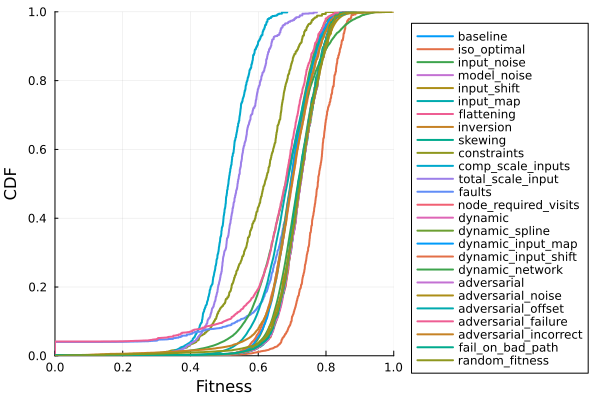
\includegraphics[width=0.97\textwidth]{test_exp_3_parallel_rnd.png}
	\caption{Experiment 3 CDF curves of fitness for best inputs using the RND optimizer while enabling individual features.}
	\label{fig:test_exp_3_parallel_rnd}
    \end{minipage}\hfill
    \begin{minipage}[t]{0.47\textwidth}
        \centering
        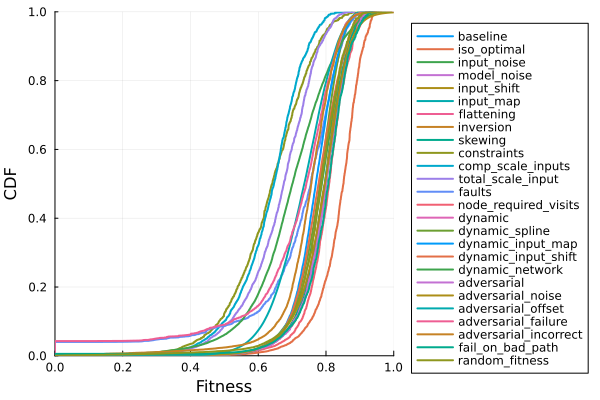
\includegraphics[width=0.97\textwidth]{test_exp_3_parallel_eca.png}
	\caption{Experiment 3 CDF curves of fitness for best inputs using the ECA optimizer while enabling individual features.}
	\label{fig:test_exp_3_parallel_eca}
    \end{minipage}
\end{figure}

\begin{figure}
	\centering
    \begin{minipage}[t]{0.47\textwidth}
        \centering
        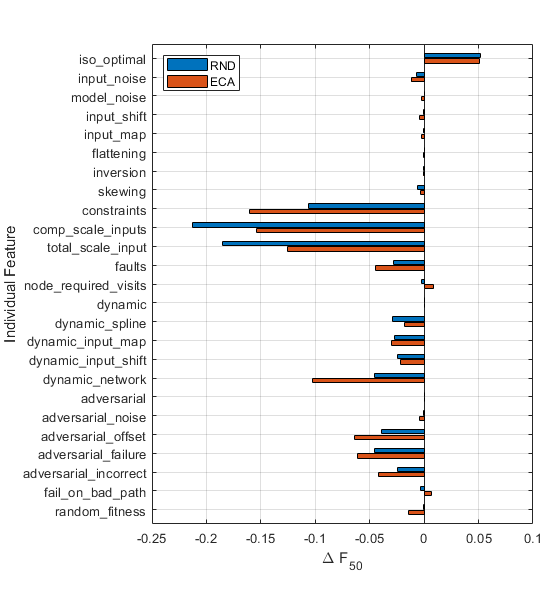
\includegraphics[width=0.97\textwidth]{test_exp_3_parallel_f50.png}
	\caption{Experiment 3 scores for $\Delta F_{50}$ for RND and ECA optimizers when enabling individual features.}
	\label{fig:test_exp_3_parallel_f50}
    \end{minipage}\hfill
    \begin{minipage}[t]{0.47\textwidth}
        \centering
        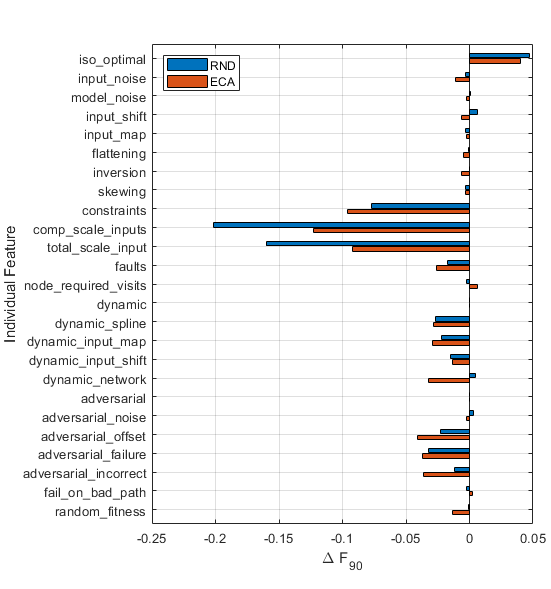
\includegraphics[width=0.97\textwidth]{test_exp_3_parallel_f90.png}
	\caption{Experiment 3 scores for $\Delta F_{90}$ for RND and ECA optimizers when enabling individual features.}
	\label{fig:test_exp_3_parallel_f90}
    \end{minipage}
\end{figure}


%--------------------------------------------------------------------------------------------
%--------------------------------------------------------------------------------------------
%--------------------------------------------------------------------------------------------

\subsubsection{Impact of Stacking Features}

Results for enabling features cumulatively in series are provided in Table \ref{tbl:exp3-series} with Figures \ref{fig:test_exp_3_series_rnd} and \ref{fig:test_exp_3_series_eca} showing CDF curve results for RND and ECA as well as Figures \ref{fig:test_exp_3_series_f50} and \ref{fig:test_exp_3_series_f90} providing bar charts for $\Delta F_{50}$ and $\Delta F_{90}$ respectively.

As with individual features, the first line in Table \ref{tbl:exp3-series} is the baseline performance with all  additional features off. The baseline and iso\_optimal lines match the results from the previous section as expected for a repeatable simulation. The performance gain from enabling the iso-optimal surface is slowly eroded when adding basic landscape and noise features from input noise through coupled pair skewing. While ECA starts with higher fitness than RND, the erosion in performance with these basic features is higher than for RND.

The first three large drops in performance are clearly visible in Figures \ref{fig:test_exp_3_series_f50} and \ref{fig:test_exp_3_series_f90} when enabling constraints, composition function scale input, and node total fitness scale input. The performance degradation while adding features is comparable for RND and ECA between adding constraints up through enabling dynamic input shifting. The dynamic network remapping has a more pronounced effect on ECA than for RND. Adversarial features generally have more of an impact on $F_{90}$ score than for $F_{50}$ as expected due to the nature of the adversarial effect to be scaled to be stronger when near more optimal performance. Lastly, the feature to enable simulation failure on invalid paths, fail\_on\_bad\_path, results in a very strong performance drop in $F_{90}$ with less so in $F_{50}$.

In general, the performance for ECA starts and stays higher than for RND as features are added up until dynamic network remapping is enabled. At which point the overall performance for ECA drops and stays nearly equivalent to RND. Ultimately for the four node four dimension scenario both optimizer's $F_{90}$ performance with all features enabled sits just above zero at 0.033 for RND and 0.023 for ECA.



\begin{table}[H]
	\centering
	\caption{Experiment 3 Fitness Sensitivity Results for Stacking Features}
	\label{tbl:exp3-series}
	\newcolumntype{C}[1]{>{\centering\arraybackslash}p{#1}}
	\begin{tabular}{| p{0.2\linewidth} | C{0.12\linewidth} | C{0.12\linewidth} | C{0.12\linewidth} | C{0.12\linewidth} | C{0.12\linewidth} | }
	\hline
	 & \multicolumn{2}{c|}{RND} & \multicolumn{2}{c|}{ECA} \\ \hline
\textbf{Features} & \textbf{$\Delta F_{50}$} & \textbf{$\Delta F_{90}$} & \textbf{$\Delta F_{50}$} & \textbf{$\Delta F_{90}$} \\ \hline


baseline & 0.723 & 0.797 & 0.799 & 0.871 \\ \hline
iso\_optimal & +0.052 & +0.047 & +0.051 & +0.040 \\ \hline
input\_noise & +0.044 & +0.042 & +0.038 & +0.031 \\ \hline
model\_noise & +0.040 & +0.037 & +0.030 & +0.022 \\ \hline
input\_shift & +0.039 & +0.031 & +0.025 & +0.021 \\ \hline
input\_map & +0.042 & +0.038 & +0.031 & +0.021 \\ \hline
flattening & +0.042 & +0.038 & +0.028 & +0.022 \\ \hline
inversion & +0.041 & +0.038 & +0.029 & +0.022 \\ \hline
skewing & +0.037 & +0.037 & +0.025 & +0.021 \\ \hline
constraints & -0.178 & -0.086 & -0.179 & -0.100 \\ \hline
comp\_scale\_inputs & -0.362 & -0.299 & -0.363 & -0.266 \\ \hline
total\_scale\_input & -0.464 & -0.413 & -0.462 & -0.383 \\ \hline
faults & -0.484 & -0.429 & -0.489 & -0.421 \\ \hline
node\_required\_visits & -0.572 & -0.507 & -0.609 & -0.482 \\ \hline
dynamic & -0.572 & -0.507 & -0.609 & -0.482 \\ \hline
dynamic\_spline & -0.591 & -0.540 & -0.616 & -0.497 \\ \hline
dynamic\_input\_map & -0.612 & -0.562 & -0.638 & -0.556 \\ \hline
dynamic\_input\_shift & -0.617 & -0.574 & -0.641 & -0.564 \\ \hline
dynamic\_network & -0.684 & -0.597 & -0.770 & -0.656 \\ \hline
adversarial & -0.684 & -0.597 & -0.770 & -0.656 \\ \hline
adversarial\_noise & -0.685 & -0.598 & -0.770 & -0.663 \\ \hline
adversarial\_offset & -0.685 & -0.602 & -0.771 & -0.666 \\ \hline
adversarial\_failure & -0.685 & -0.602 & -0.771 & -0.665 \\ \hline
adversarial\_incorrect & -0.686 & -0.592 & -0.763 & -0.671 \\ \hline
fail\_on\_bad\_path & -0.724 & -0.765 & -0.800 & -0.849 \\ \hline
random\_fitness & -0.724 & -0.765 & -0.800 & -0.849 \\ \hline


	\end{tabular}
\end{table}




\begin{figure}
	\centering
    \begin{minipage}[t]{0.47\textwidth}
        \centering
        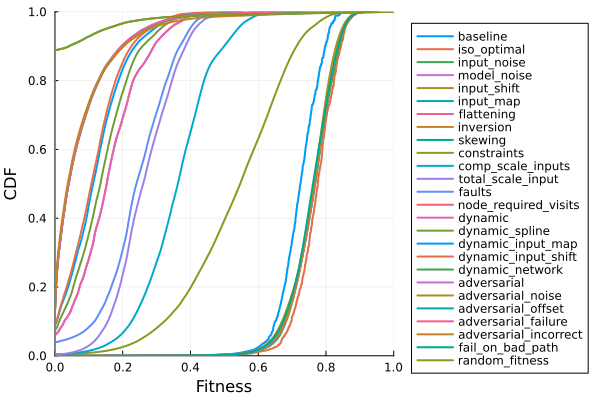
\includegraphics[width=0.97\textwidth]{test_exp_3_series_rnd.png}
	\caption{Experiment 3 CDF curves of fitness for best inputs using the RND optimizer while progressively including features.}
	\label{fig:test_exp_3_series_rnd}
    \end{minipage}\hfill
    \begin{minipage}[t]{0.47\textwidth}
        \centering
        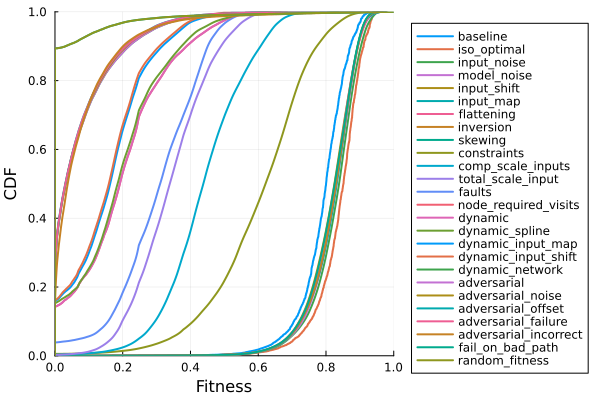
\includegraphics[width=0.97\textwidth]{test_exp_3_series_eca.png}
	\caption{Experiment 3 CDF curves of fitness for best inputs using the ECA optimizer while progressively including features.}
	\label{fig:test_exp_3_series_eca}
    \end{minipage}
\end{figure}


\begin{figure}
	\centering
    \begin{minipage}[t]{0.47\textwidth}
        \centering
        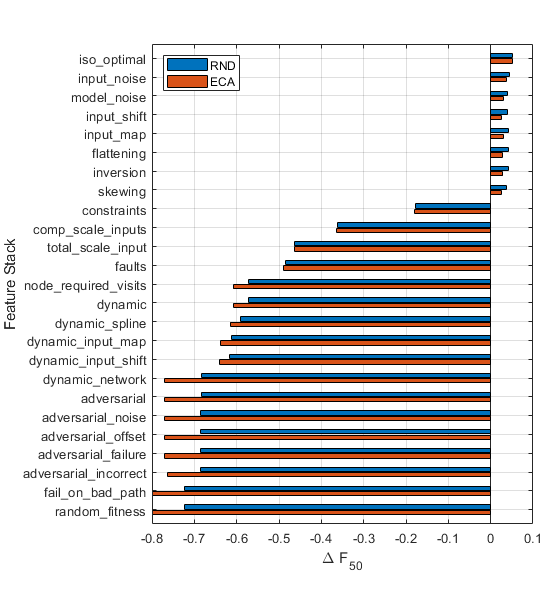
\includegraphics[width=0.97\textwidth]{test_exp_3_series_f50.png}
	\caption{Experiment 3 scores for $\Delta F_{50}$ for RND and ECA optimizers with cumulative features.}
	\label{fig:test_exp_3_series_f50}
    \end{minipage}\hfill
    \begin{minipage}[t]{0.47\textwidth}
        \centering
        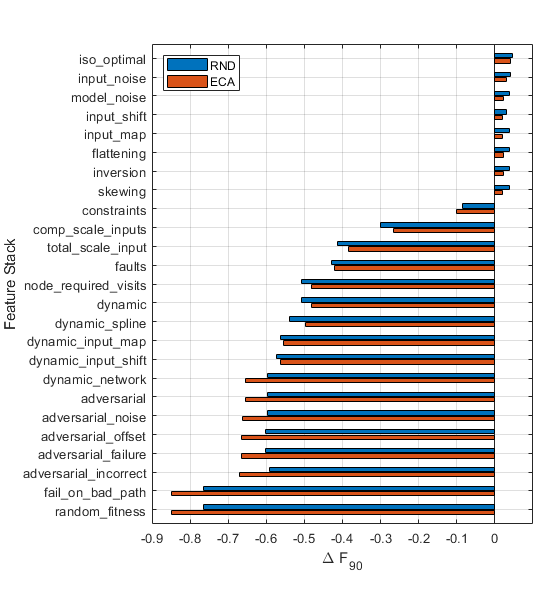
\includegraphics[width=0.97\textwidth]{test_exp_3_series_f90.png}
	\caption{Experiment 3 scores for $\Delta F_{90}$ for RND and ECA optimizers with cumulative features.}
	\label{fig:test_exp_3_series_f90}
    \end{minipage}
\end{figure}

%--------------------------------------------------------------------------------------------
%--------------------------------------------------------------------------------------------
%--------------------------------------------------------------------------------------------



\section{Conclusions}

This paper started with a review of optimization, in particular approaches that use heuristics, meta-heuristics, and hyper-heuristics. The close relationship between simulation and optimization was explored to include their importance to engineering design optimization in the face of uncertainty as well as their use in decision analysis and robust decision making under varying levels uncertainty. This was then used to related robust decision making to overcoming adversarial surprise, unanticipated consequences to decisions, and analogs to hyper-heuristic optimization strategies.

Next, a review was provided on the importance of benchmarking and computational experimentation of algorithms. This included important advancements in optimization algorithm performance testing. Key features of optimization problems were identified and placed in historical perspective using popular test suites. A large section was devoted to exploring the Congress of Evolutionary Computing (CEC) and Genetic and Evolutionary Computation Conference (GECCO) challenge problems that are frequently used for testing meta-heuristic algorithms. The problems have a long history and breadth of benchmarking features. Limitations were identified and used to justify the development of the Crucible Simulation for providing a highly configurable black box test suite for enhanced difficulty with adversarial and semi-cooperative features.

Requirements for simulation features were derived and traced to literature references. The simulation architecture and features were then described in detail and traced to requirements. The simulation is fundamentally a mixed-integer problem requiring pathfinding and single target optimization with scalable objective dimensionality and network size. The features include composition functions, non-axis alignment, non-separability, feasibility constraints, continuous and discrete event dynamic effects, stochasticity of inputs and responses, variable model fidelity, and a wide variety of landscape features. An important contribution of this work is the inclusion of adversarial feedback to optimizer decision making as well as semi-cooperative unexpected consequences by abruptly failing execution or enhancing stochastic optimization difficulty by returning random feasible or infeasible results. A discussion of simulation configuration parameters and justification for default values was provided.

Three experiments were defined and performed to evaluate optimizer performance while sweeping dimensionality and network size with features off and on. Experiments included ten replicates of thirty scenario seeds with ten-thousand iterations each for a total of three-million runs per treatment. CDF curves of performance were provided and the 50th and 90th percentile fitness scores, $F_{50}$ and $F_{90}$, were used for direct comparison.

Experiment 1 compared the performance between the Evolutionary Centers Algorithm (ECA), Particle Swarm Optimization (PSO), Simulated Annealing (SA), and Random Search (RND) algorithms for a scenario with one node and one, three, five, ten, and twenty dimensions. ECA, PSO, and SA dominated RND performance with all features off. ECA and PSO were nearly equivalent with PSO outperforming at the higher dimensions. PSO and SA were equivalent for one dimension, however SA dominated all others for the higher dimensions tested. A drastic performance drop appeared when including all simulation features. Contrary to the first set with all features off, PSO and SA performed markedly worse than RND and ECA with all features on. Interestingly, while ECA dominates PSO and SA, it only performed marginally better than RND for each dimension.

Experiment 2 compared the performance between ECA and RND optimization for scenarios with four dimensions and one, two, three, four, and five nodes in random networks. ECA showed marginally better performance than RND for a single node, however the improvement was much greater when more nodes were included in the network. Interestingly, ECA only showed marginally better performance than RND across all node combinations. Both RND and ECA had an $F_{90}$ score just above 0.0 at 0.033 and 0.023 respectively for four nodes. Both optimizers resulted in a 0.0 $F_{90}$ score for five nodes with four dimensions.

Experiment 3 compared the performance between ECA and RND in challenging four node, four dimension scenarios in two phases. The first phase enabled simulation features individually, then the second phase enabled features in series to evaluate their cumulative effect. For the first individual phase, enabling iso-optimal surfaces provides a large expected improvement in performance by creating many large non-convex continuous and disconnected regions with an optimal score of 1.0. Enabling input noise added uncertainty to the decision variables resulting in uncertainty propagation through the simulation calculations resulting in a noticeable drop. Many features provided negligible impact to performance as they are primarily used to create landscape variation, non-separability, and add output uncertainty. Large drops in performance were found when enabling feasibility constraints, additional scaling dimensions, and dynamic features. Adversarial features contributed additional meaningful drops in performance. For these scenarios, the ECA optimizer clearly outperformed RND.

For the second cumulative effect phase, ECA starts with higher fitness than RND, but has faster erosion in performance as basic features are added.  The first three large drops in performance were clearly visible when enabling constraints, composition function scale input, and node total fitness scale input. The performance degradation while adding features was comparable for RND and ECA between adding constraints up through enabling dynamic input shifting.  The dynamic network remapping had a more pronounced effect on ECA than for RND. Adversarial features generally had more of an impact on the $F_{90}$ scores than for $F_{50}$ as expected due to the nature of the adversarial effect to be scaled to be stronger when near more optimal performance. Lastly, the feature to enable simulation failure on invalid paths, fail\_on\_bad\_path, resulted in a very strong performance drop in $F_{90}$ with less so in $F_{50}$. In general, the performance for ECA started and stayed higher than for RND as features were added up until dynamic network remapping was enabled. At which point the overall performance for ECA dropped and stayed nearly equivalent to RND. Ultimately for the four node four dimension scenario both optimizer's $F_{90}$ performance with all features enabled sits just above zero at 0.033 for RND and 0.023 for ECA.

These experiments showed the strength of the ECA, PSO, and SA algorithms at single target optimization compared to random search. With all extra simulation features off, SA dominated RND, ECA, and PSO with one node and many dimensions. However, when all features were on, RND and ECA outperformed SA and PSO. Moreover, in the challenging all feature, four node, four dimension scenarios the high performance of ECA was eroded such that ECA and RND performed equivalently. These results motivate exploring more advanced hyper-heuristic strategies with the Crucible simulation.

\section{Acknowledgments}

The author would like to thank Dr. Ghaith Rabadi and Dr. Bulent Soykan for providing helpful feedback and recommendations during the project ideation, literature review, requirements derivation, and experiments.

\bibliography{mybib,cec}
\bibliographystyle{ieeetr}


\end{document}